\subsection{Lab1: Primeros pasos}
%*********************
\begin{frame}{}

\pgfdeclareimage[width=\paperwidth,height=\paperheight]{bg}{imagenes/fondo_lab}
\setbeamertemplate{background}{\pgfuseimage{bg}}

\bfseries{\textrm{\LARGE Lab1\\ \Large Primeros pasos}}
\raggedright
\end{frame}
%*********************

\begin{frame}{Primeros pasos}

\pgfdeclareimage[width=\paperwidth,height=\paperheight]{bg}{imagenes/fondo3}
\setbeamertemplate{background}{\pgfuseimage{bg}}

\begin{figure}[H]
\centering
\vspace{-3mm}
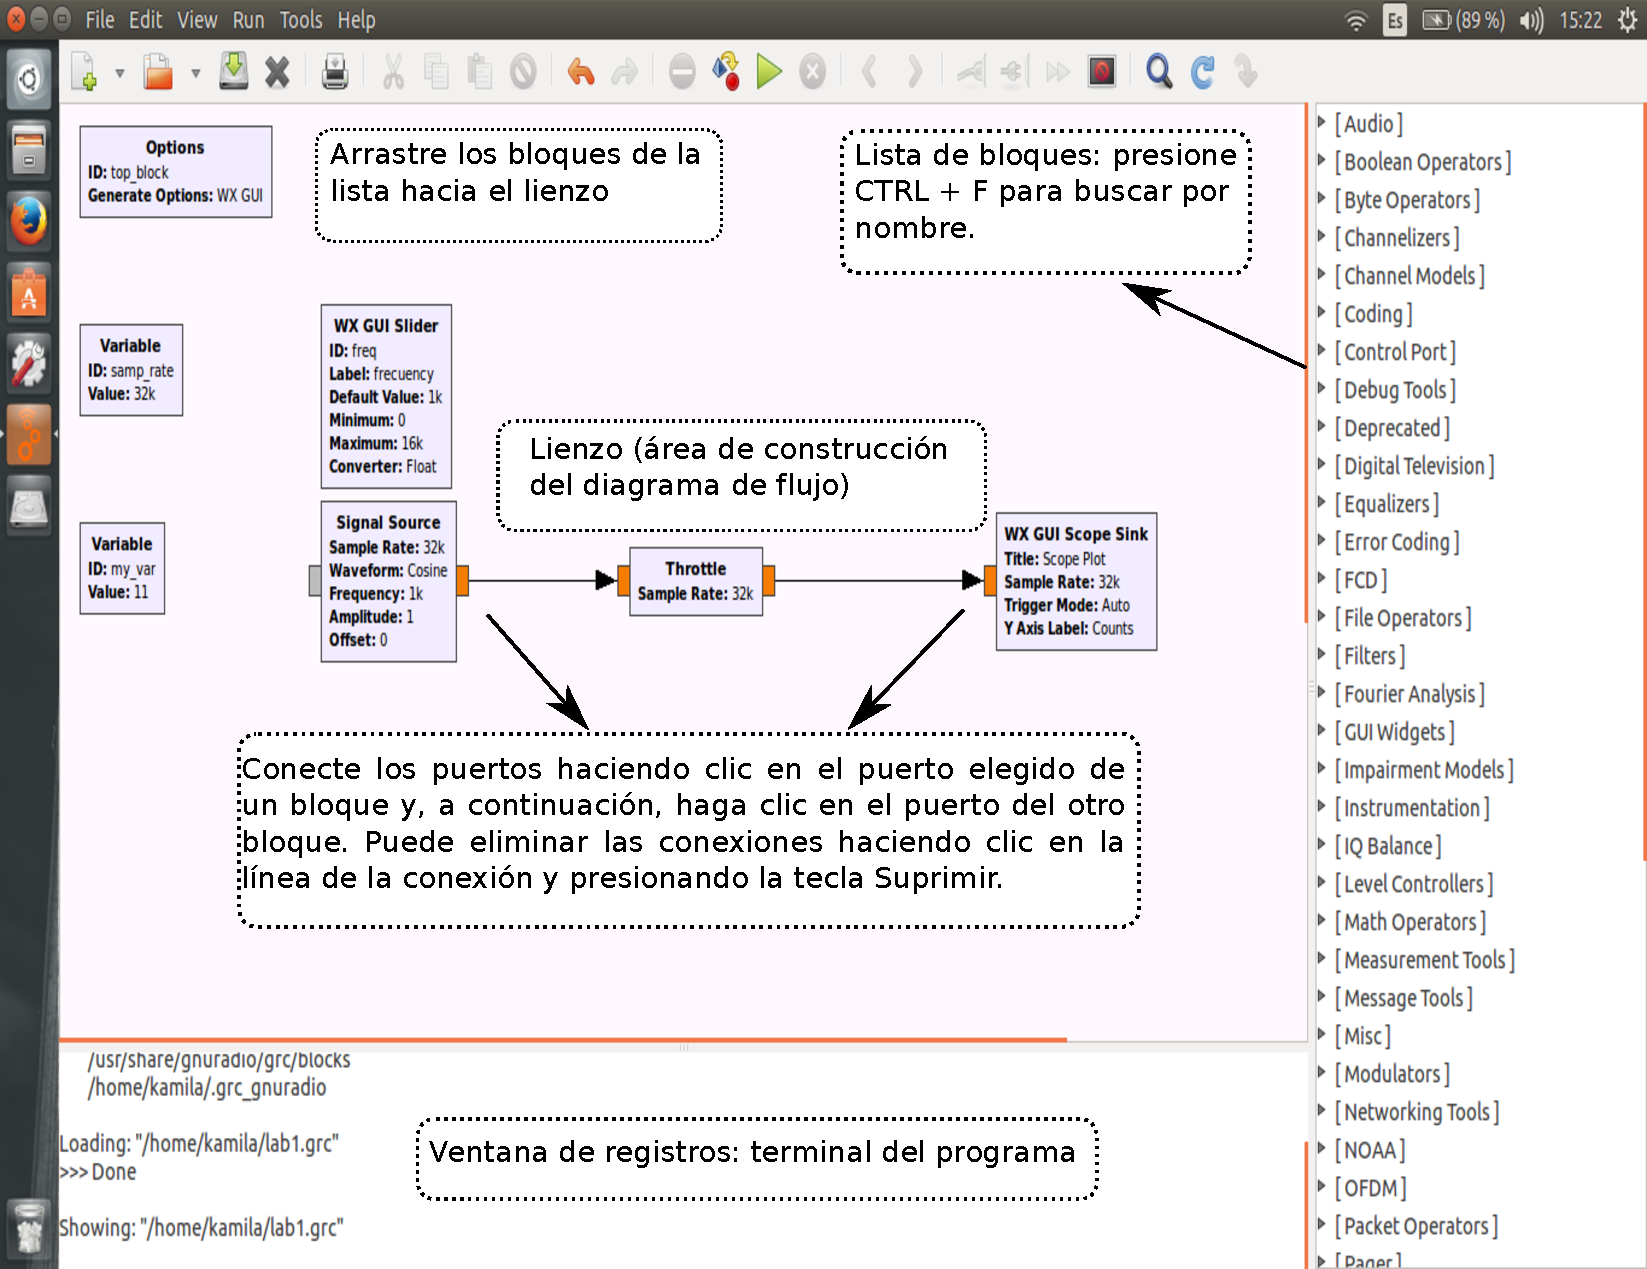
\includegraphics[width=0.9\textwidth]{parte1/lab1/pdf/lab1_1.pdf}
\end{figure}
\end{frame}
%-----------------------------------

\begin{frame}{Primeros pasos }
\begin{figure}[H]
\centering
\vspace{-3mm}
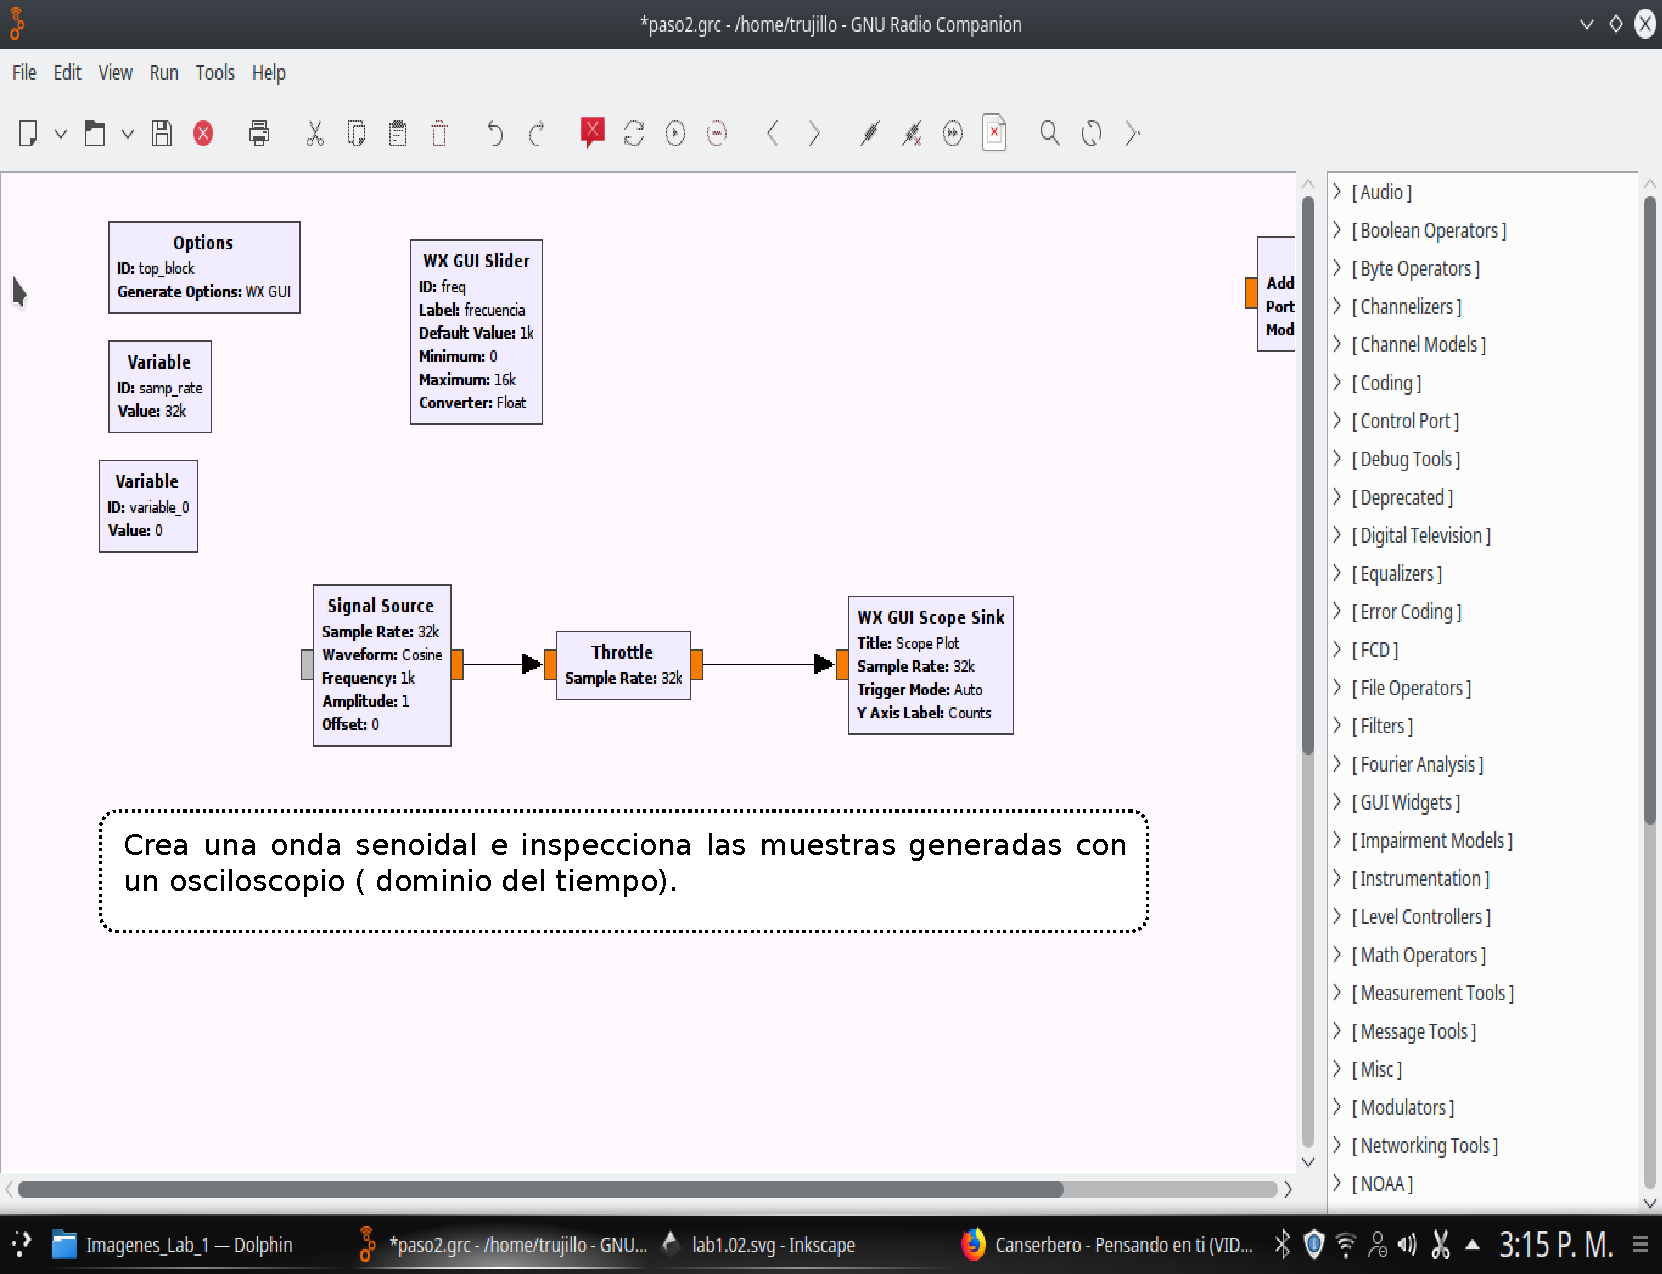
\includegraphics[width=0.9\textwidth]{parte1/lab1/pdf/lab1_2.pdf}
\end{figure}
\end{frame}
%-----------------------------------

\begin{frame}{Primeros pasos }
\begin{figure}[H]
\vspace{-3mm}
\centering
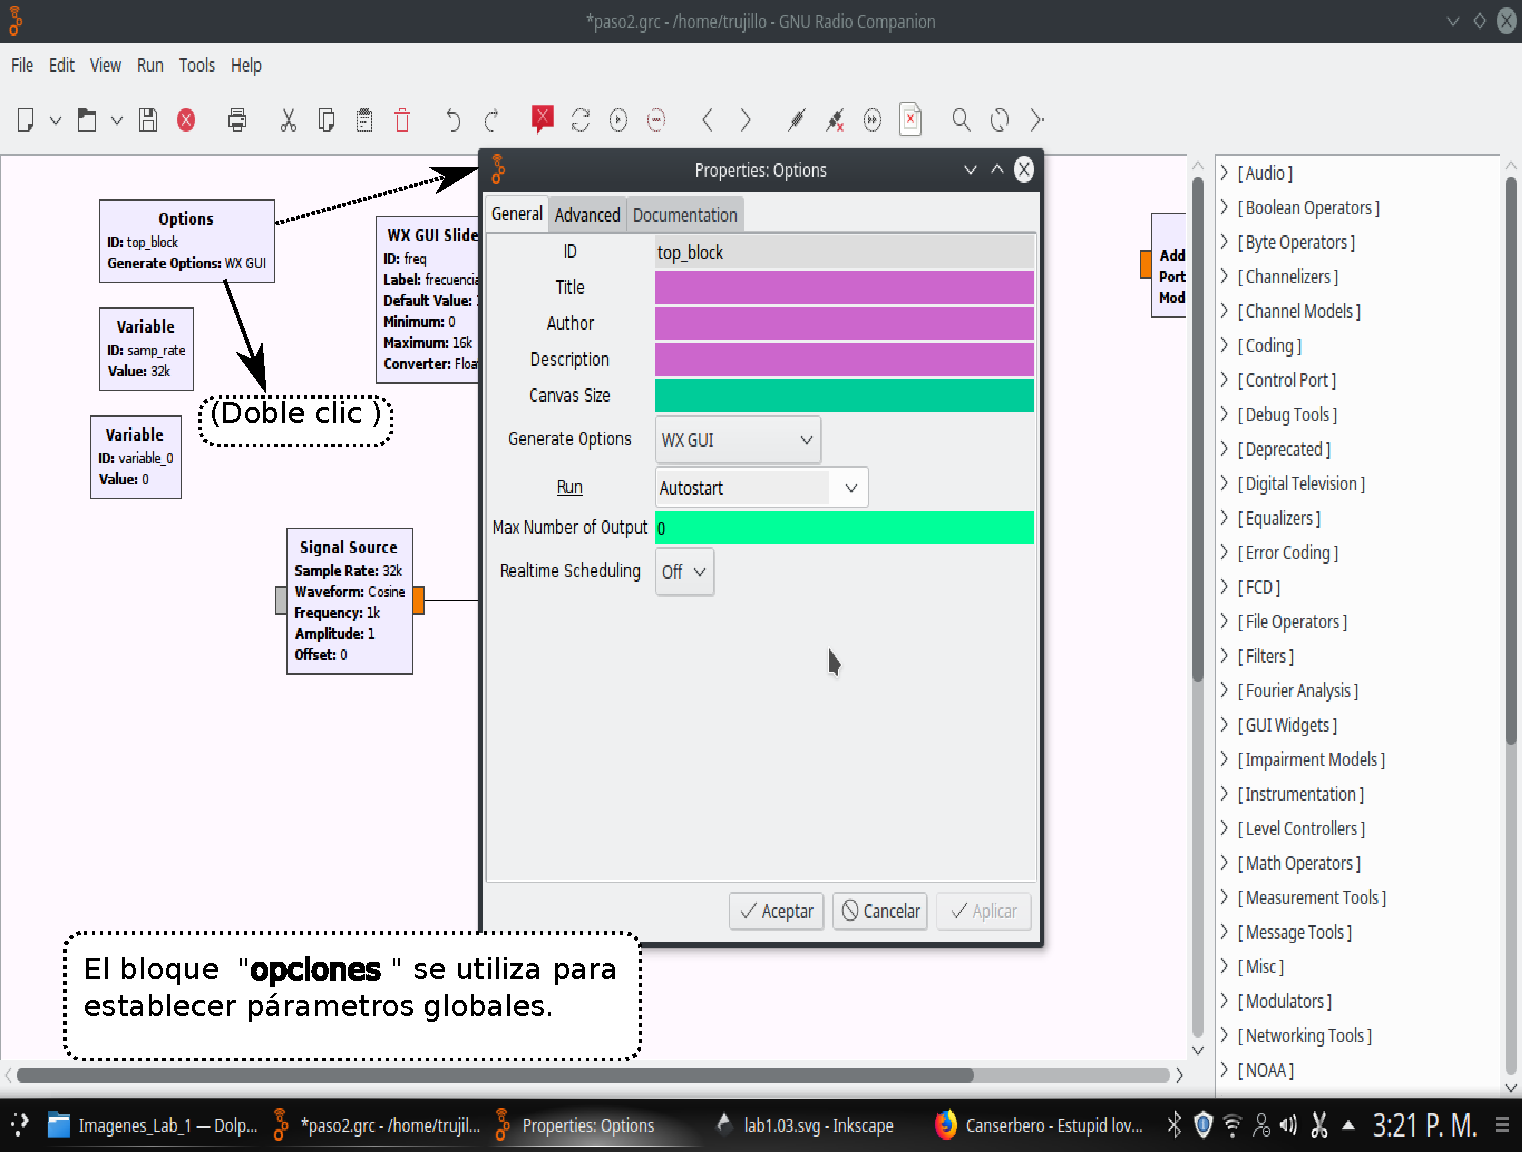
\includegraphics[width=0.9\textwidth]{parte1/lab1/pdf/lab1_3.pdf}
\end{figure}
\end{frame}
%-----------------------------------

\begin{frame}{Primeros pasos }
\begin{figure}[H]
\vspace{-3mm}
\centering
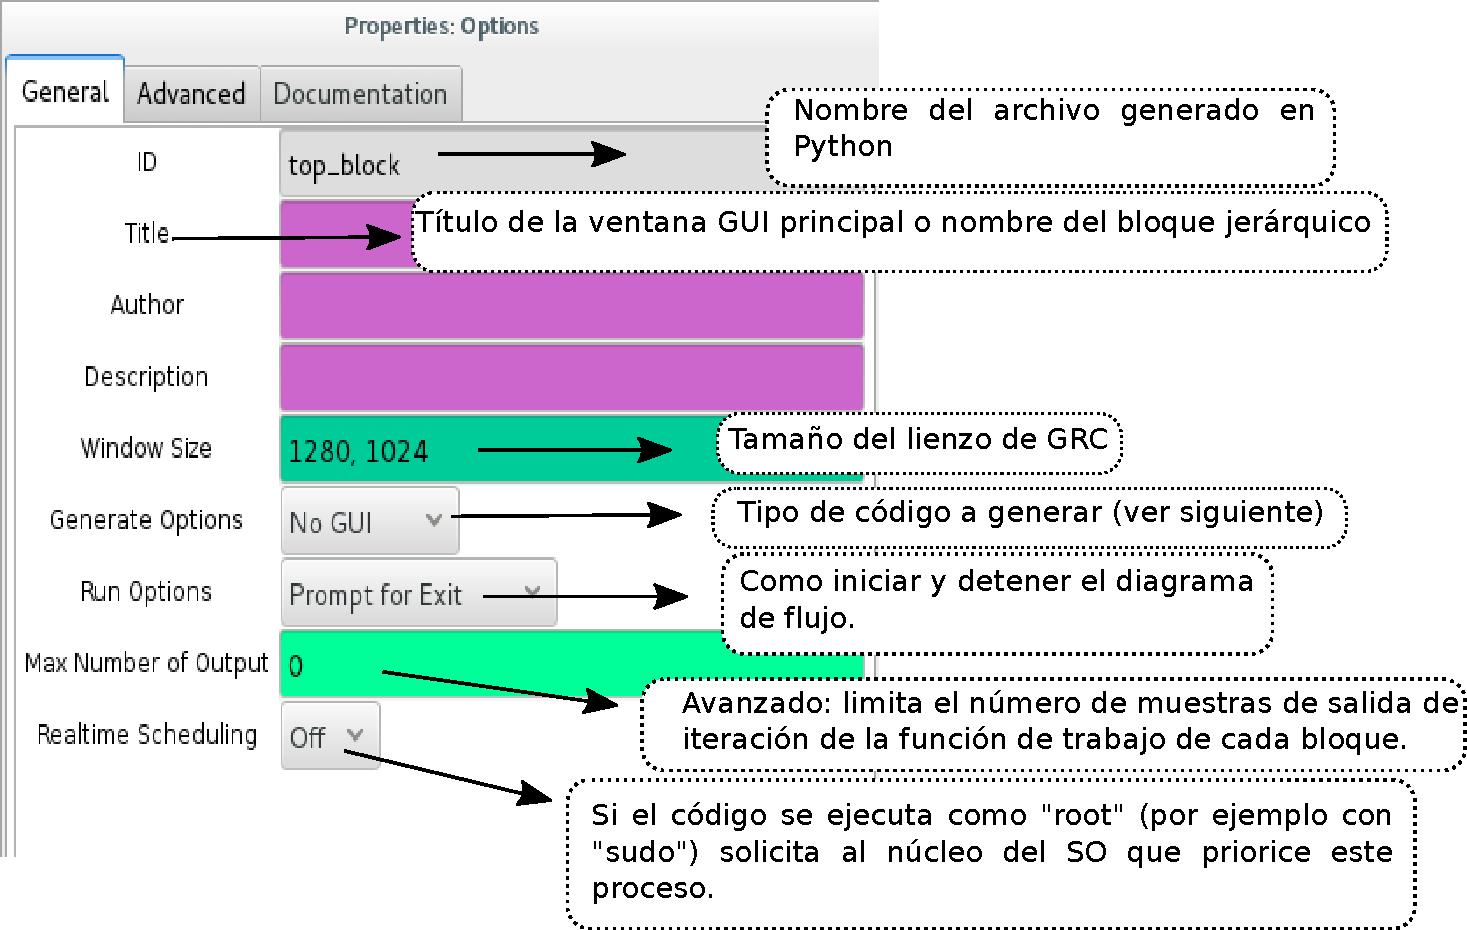
\includegraphics[width=0.9\textwidth]{parte1/lab1/pdf/lab1_4.pdf}
\end{figure}
\end{frame}
%-----------------------------------

\begin{frame}{Primeros pasos }
\begin{figure}[H]
\vspace{-2cm}
\centering
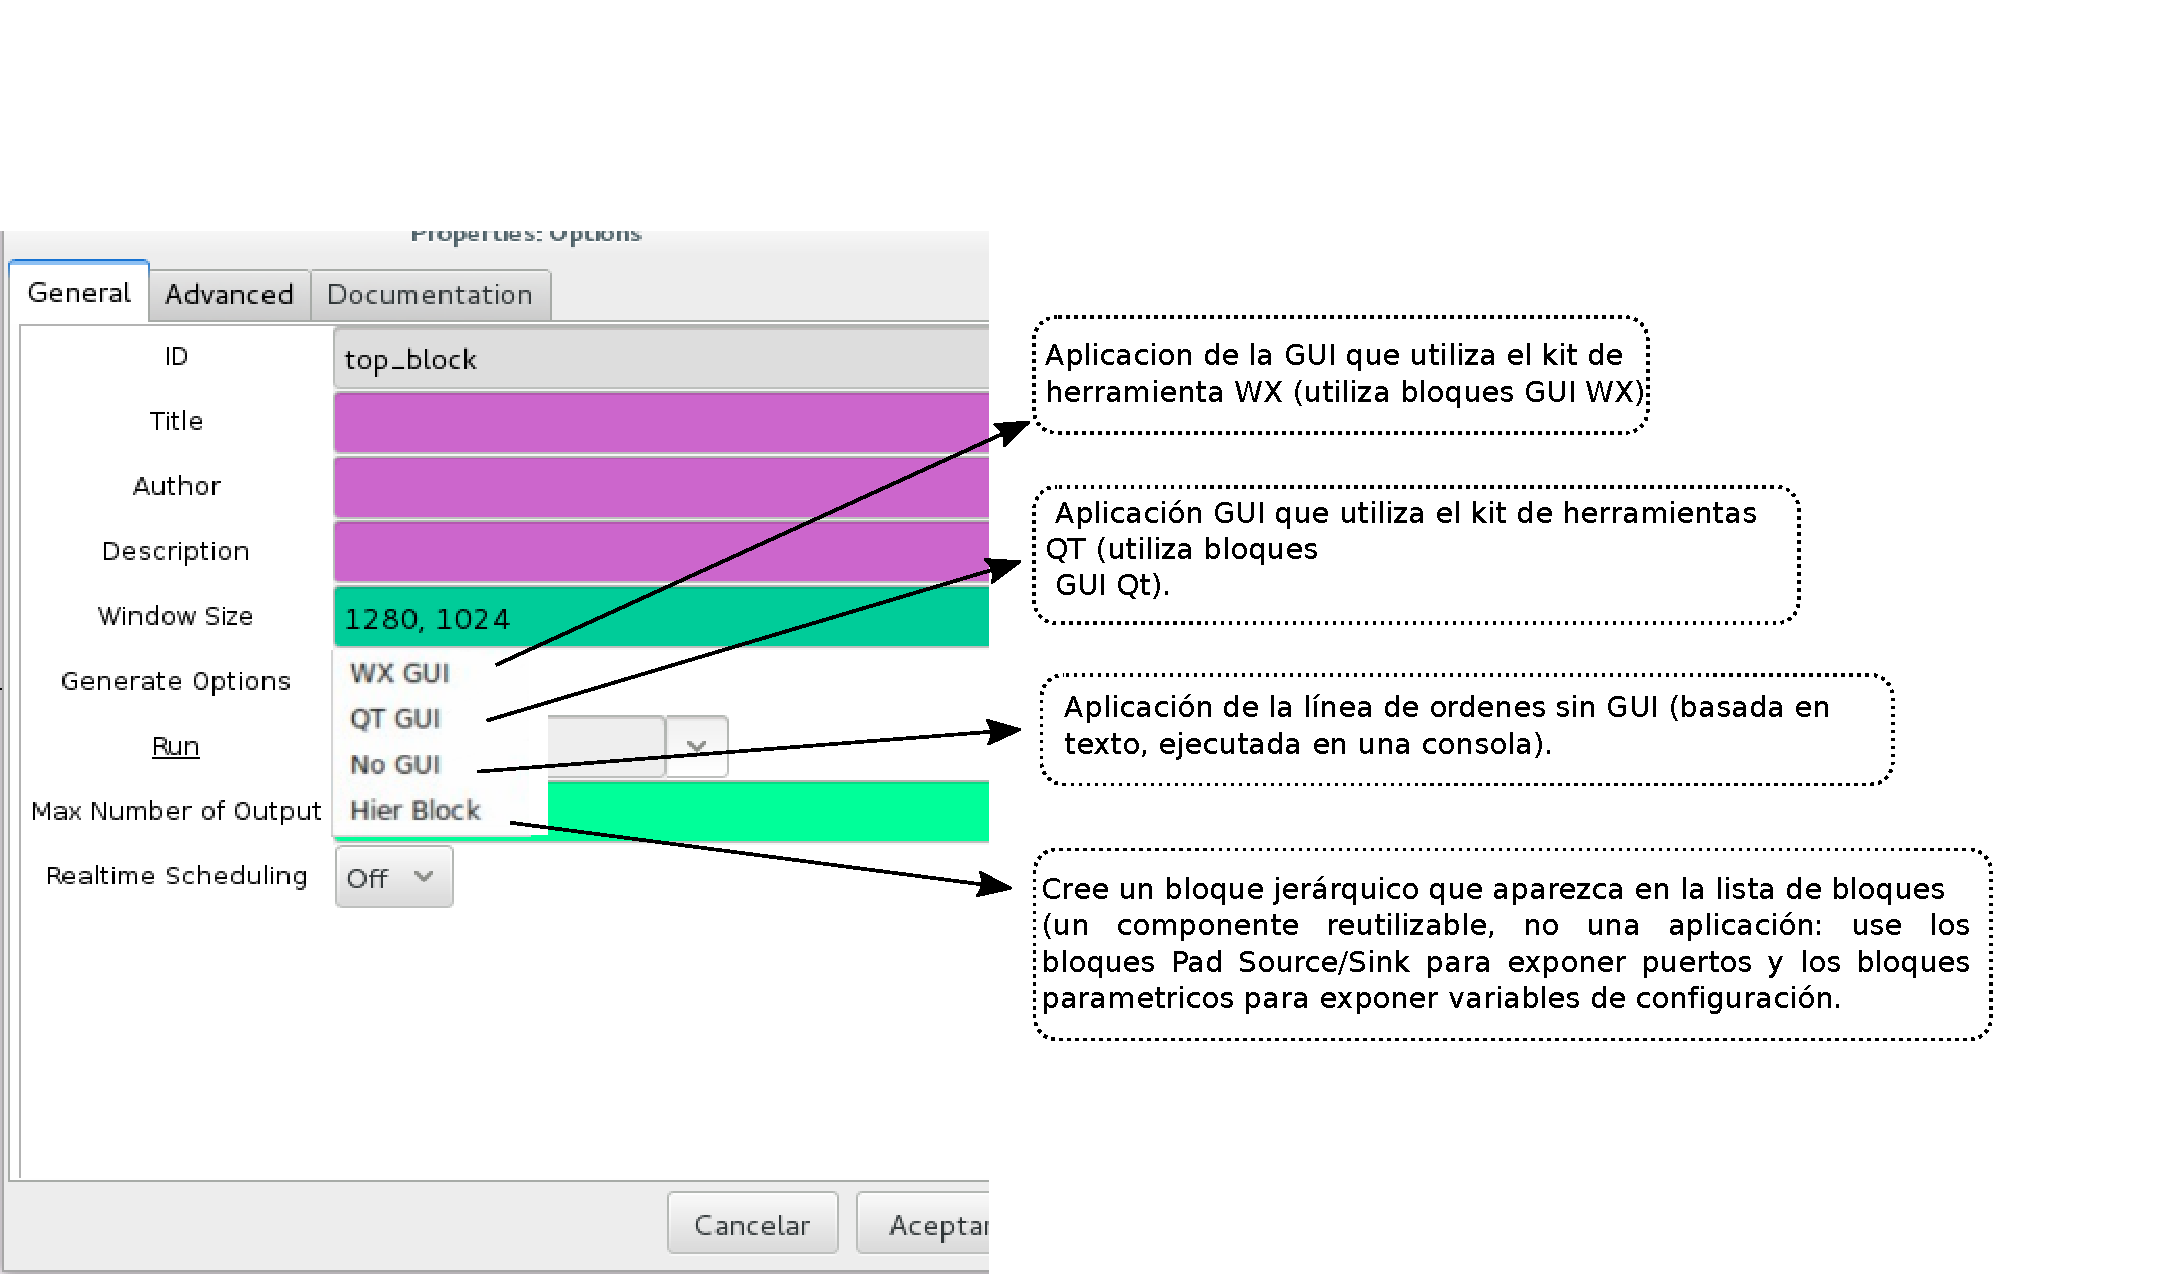
\includegraphics[width=1.1\textwidth]{parte1/lab1/pdf/lab1_5.pdf}
\end{figure}
\end{frame}
%-----------------------------------

\begin{frame}{Primeros pasos }
\begin{figure}[H]
\centering
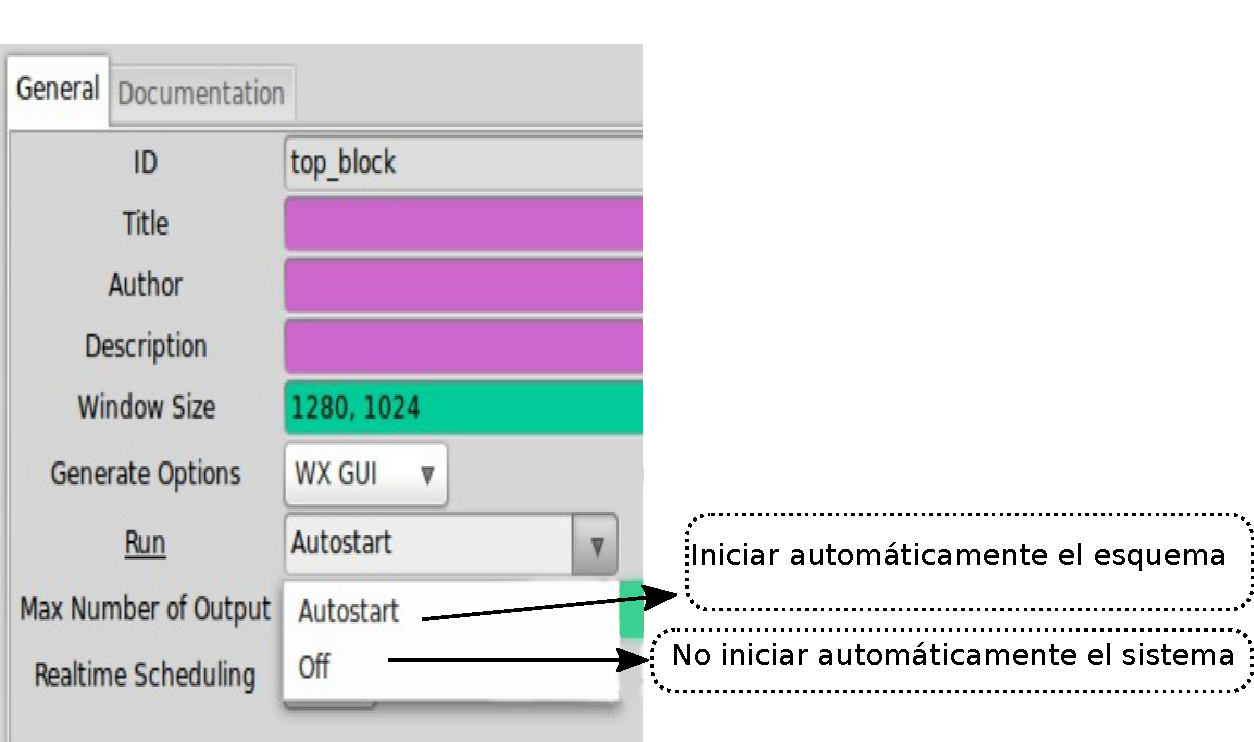
\includegraphics[width=.9\textwidth]{parte1/lab1/pdf/lab1_6.pdf}
\end{figure}
\end{frame}
%-----------------------------------

\begin{frame}{Primeros pasos }
\begin{figure}[H]
\centering
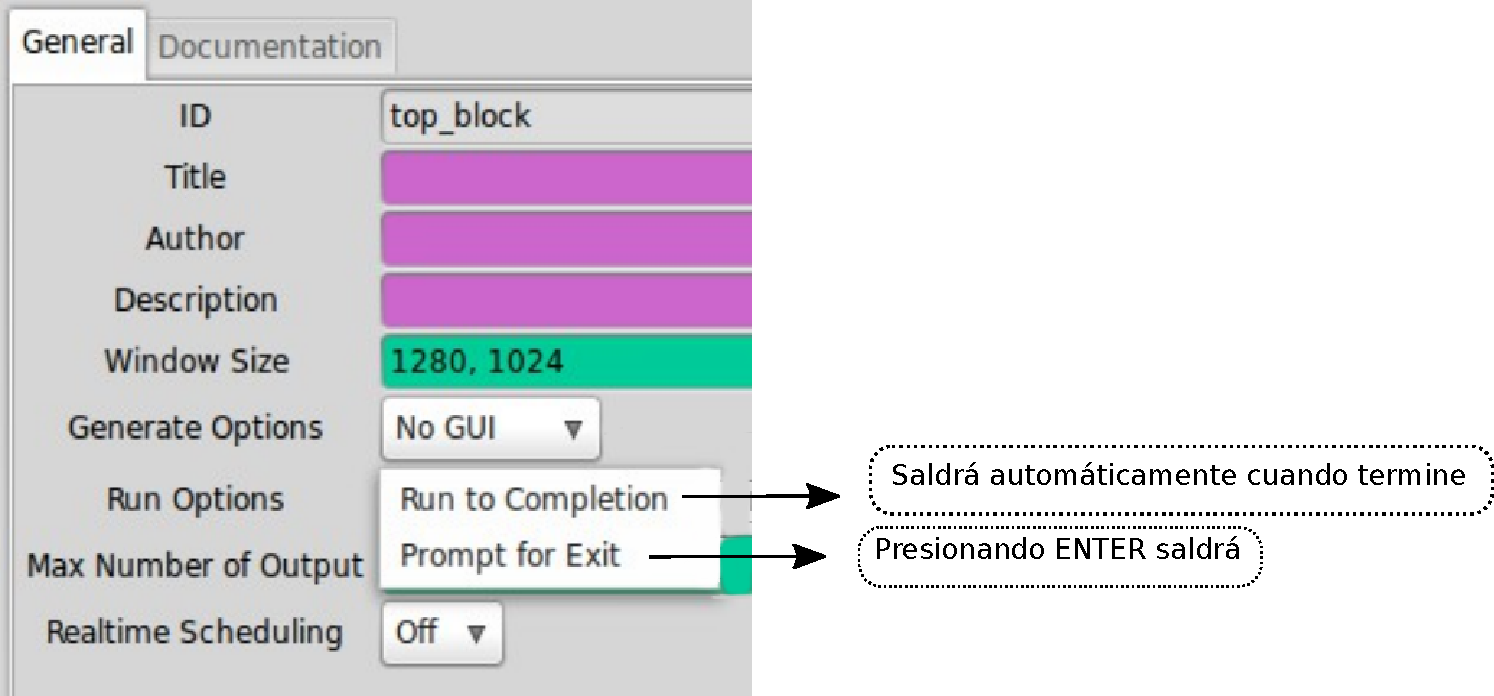
\includegraphics[width=\textwidth]{parte1/lab1/pdf/lab1_7.pdf}
\end{figure}
\end{frame}
%-----------------------------------

\begin{frame}{Primeros pasos }
\begin{figure}[H]
\vspace{-1cm}
\centering
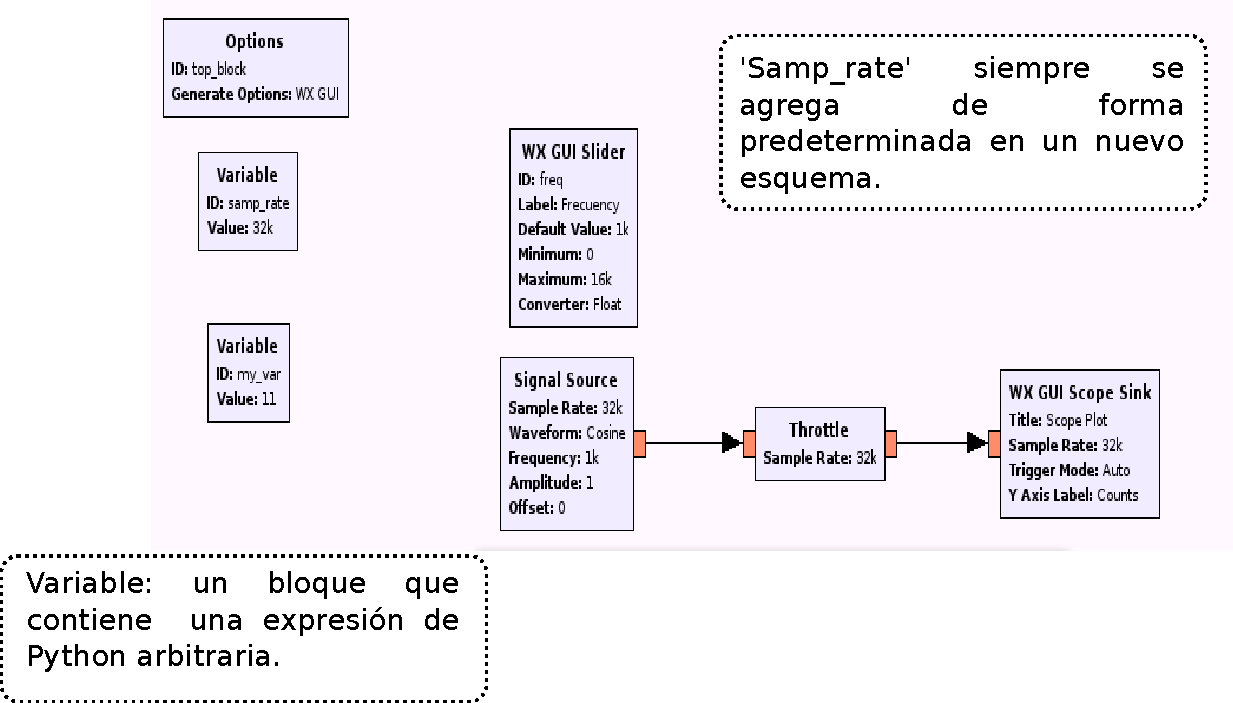
\includegraphics[width=\textwidth]{parte1/lab1/pdf/lab1_8.pdf}
\end{figure}
\end{frame}
%-----------------------------------

\begin{frame}{Primeros pasos }
\begin{figure}[H]
\vspace{-3mm}
\centering
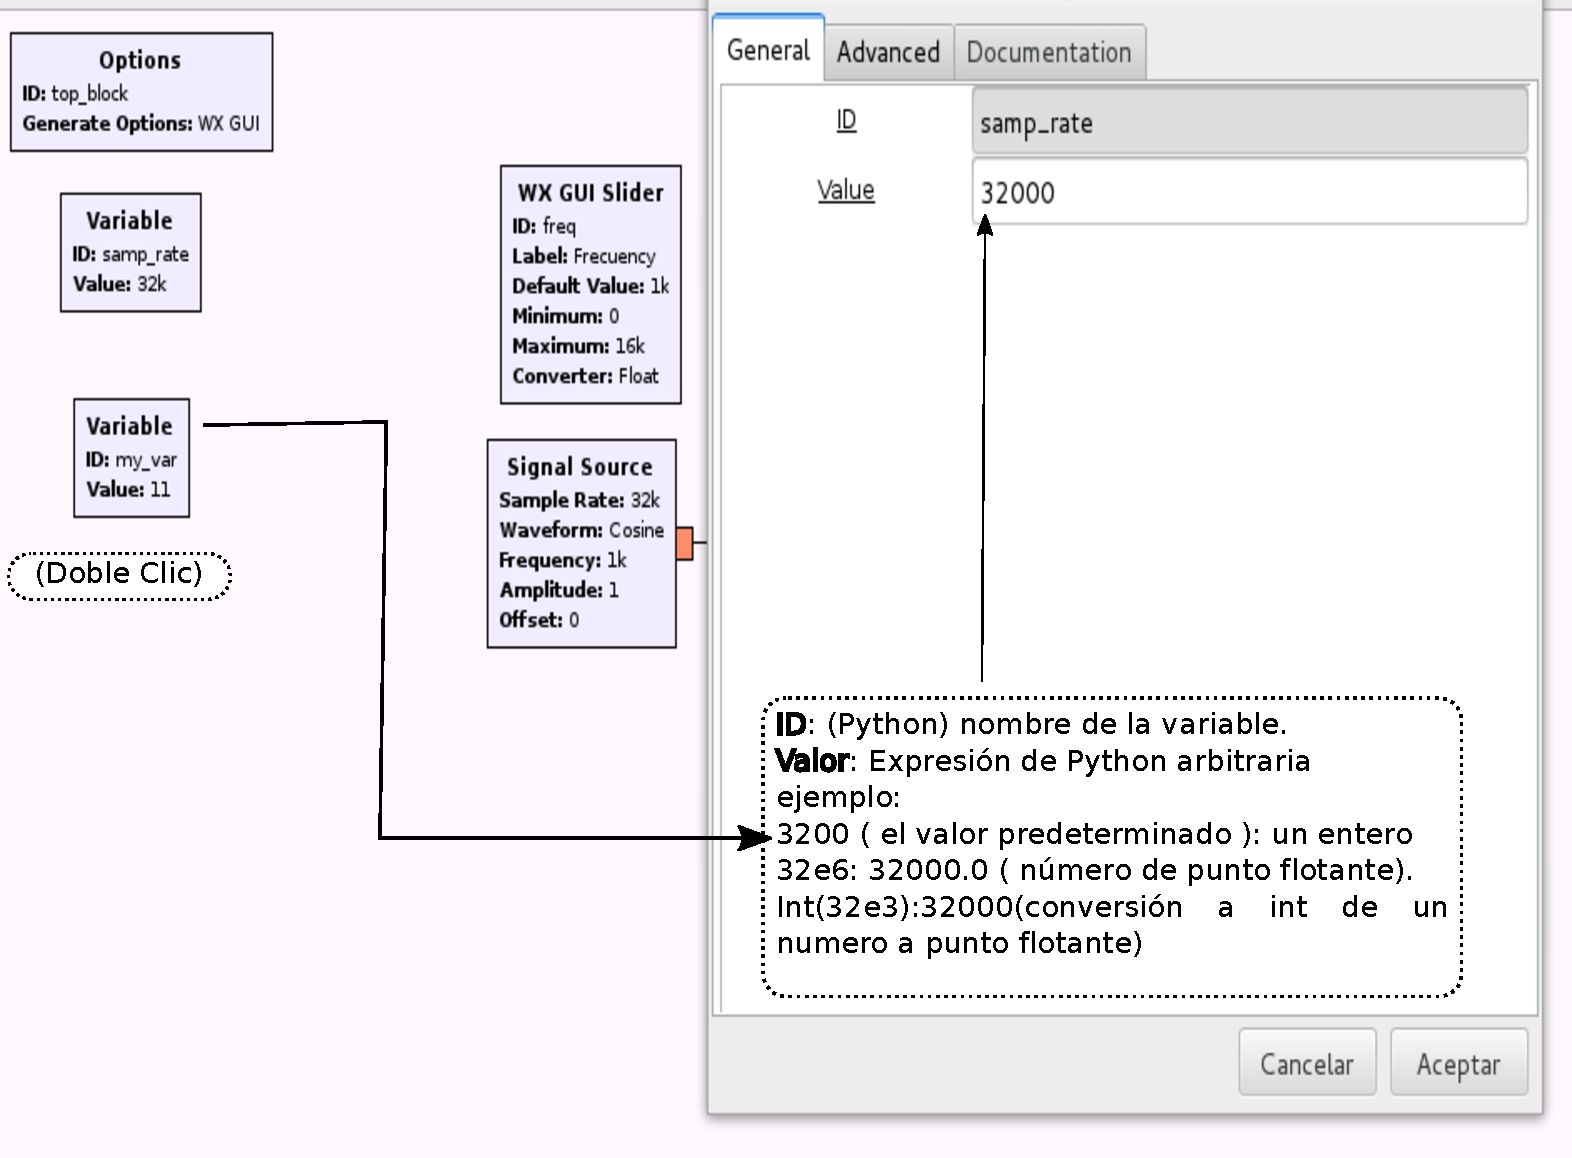
\includegraphics[width=0.85\textwidth]{parte1/lab1/pdf/lab1_9.pdf}
\end{figure}
\end{frame}
%-----------------------------------

\begin{frame}{Primeros pasos }
\begin{figure}[H]
\vspace{-3mm}
\centering
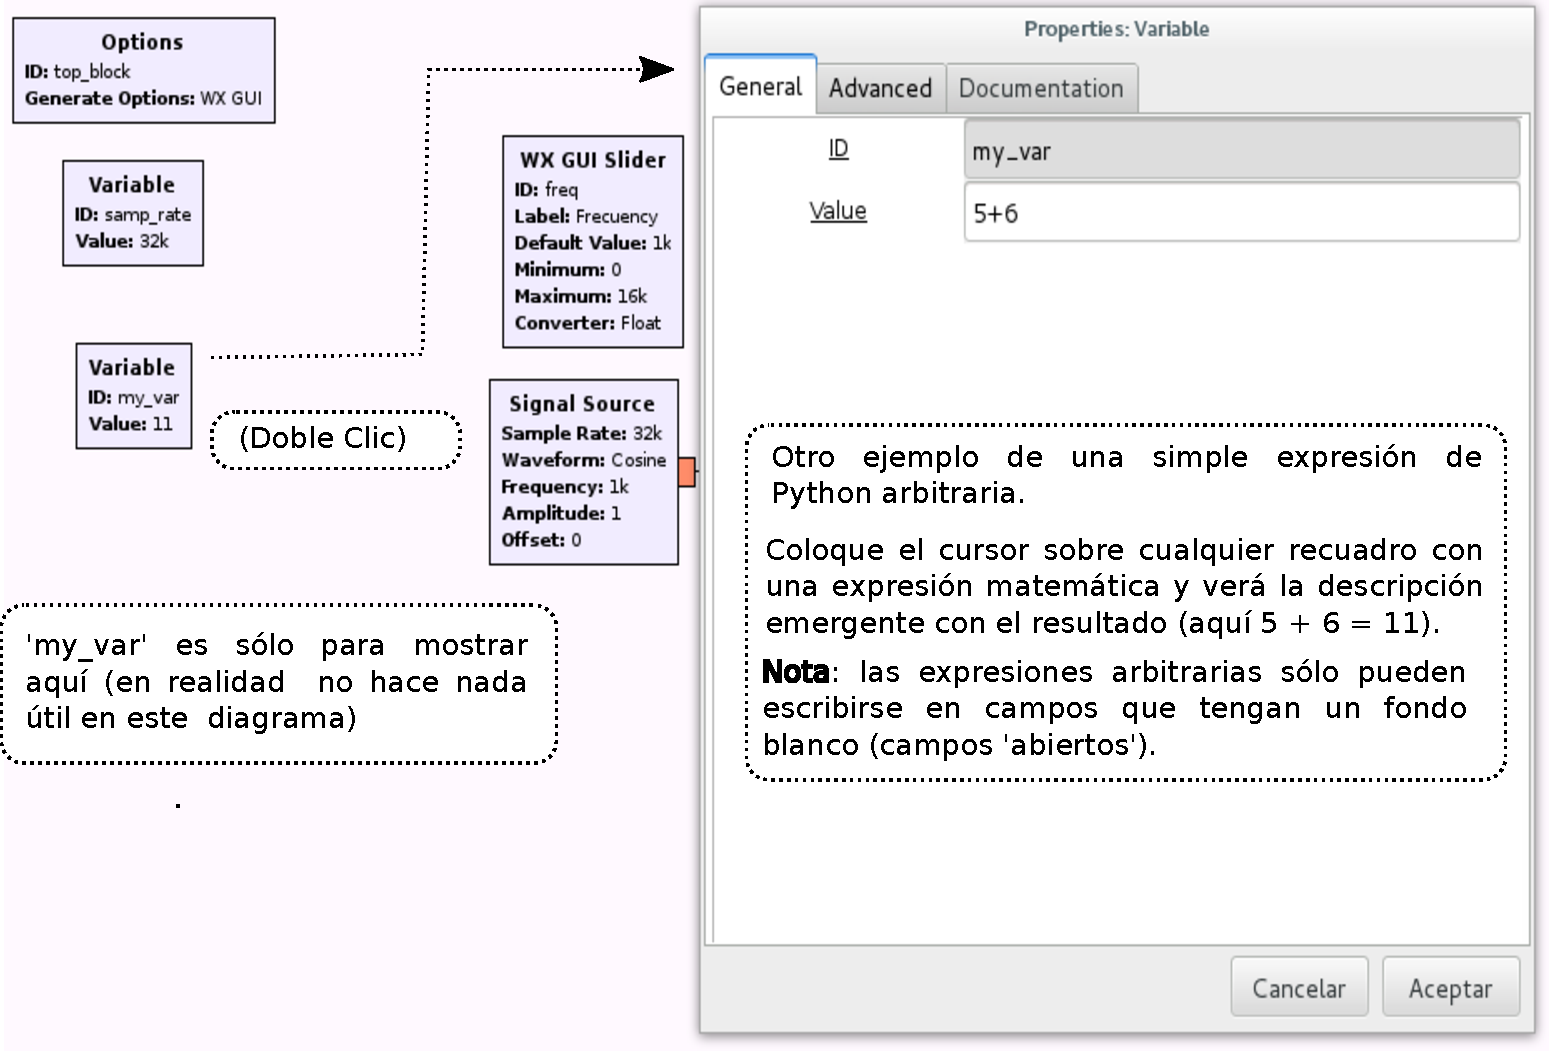
\includegraphics[width=.9\textwidth]{parte1/lab1/pdf/lab1_10.pdf}
\end{figure}
\end{frame}
%-----------------------------------

\begin{frame}{Primeros pasos }
\begin{figure}[H]
\vspace{-3mm}
\centering
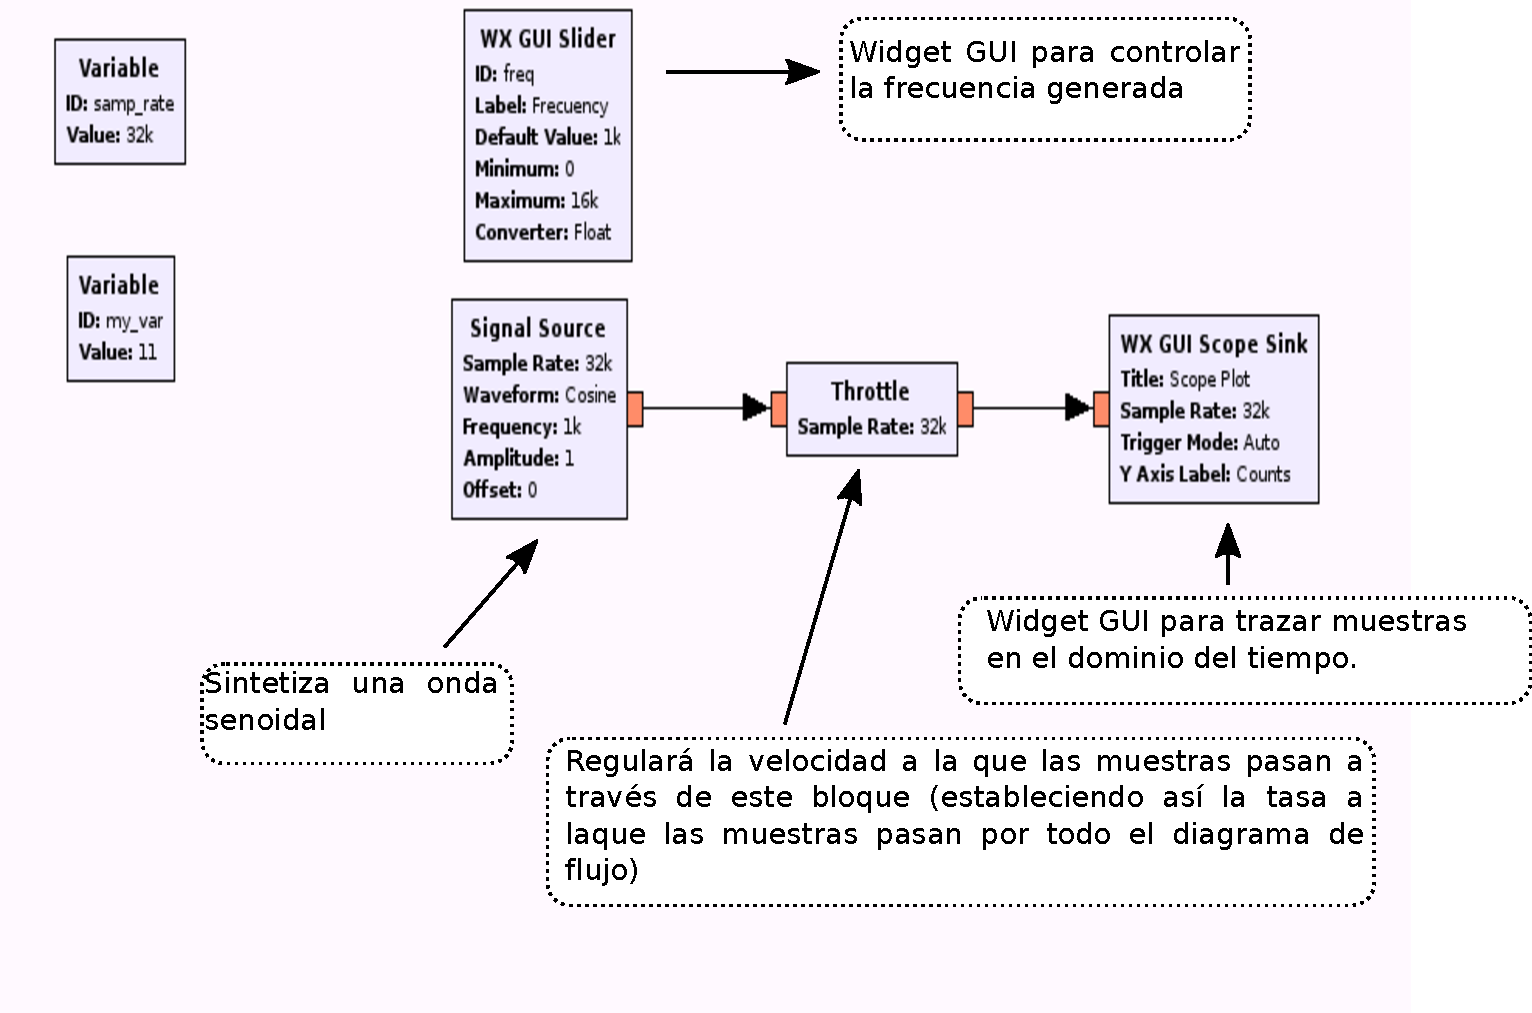
\includegraphics[width=\textwidth]{parte1/lab1/pdf/lab1_11.pdf}
\end{figure}
\end{frame}
%-----------------------------------

\begin{frame}{Primeros pasos }
\begin{figure}[H]
\vspace{-3mm}
\centering
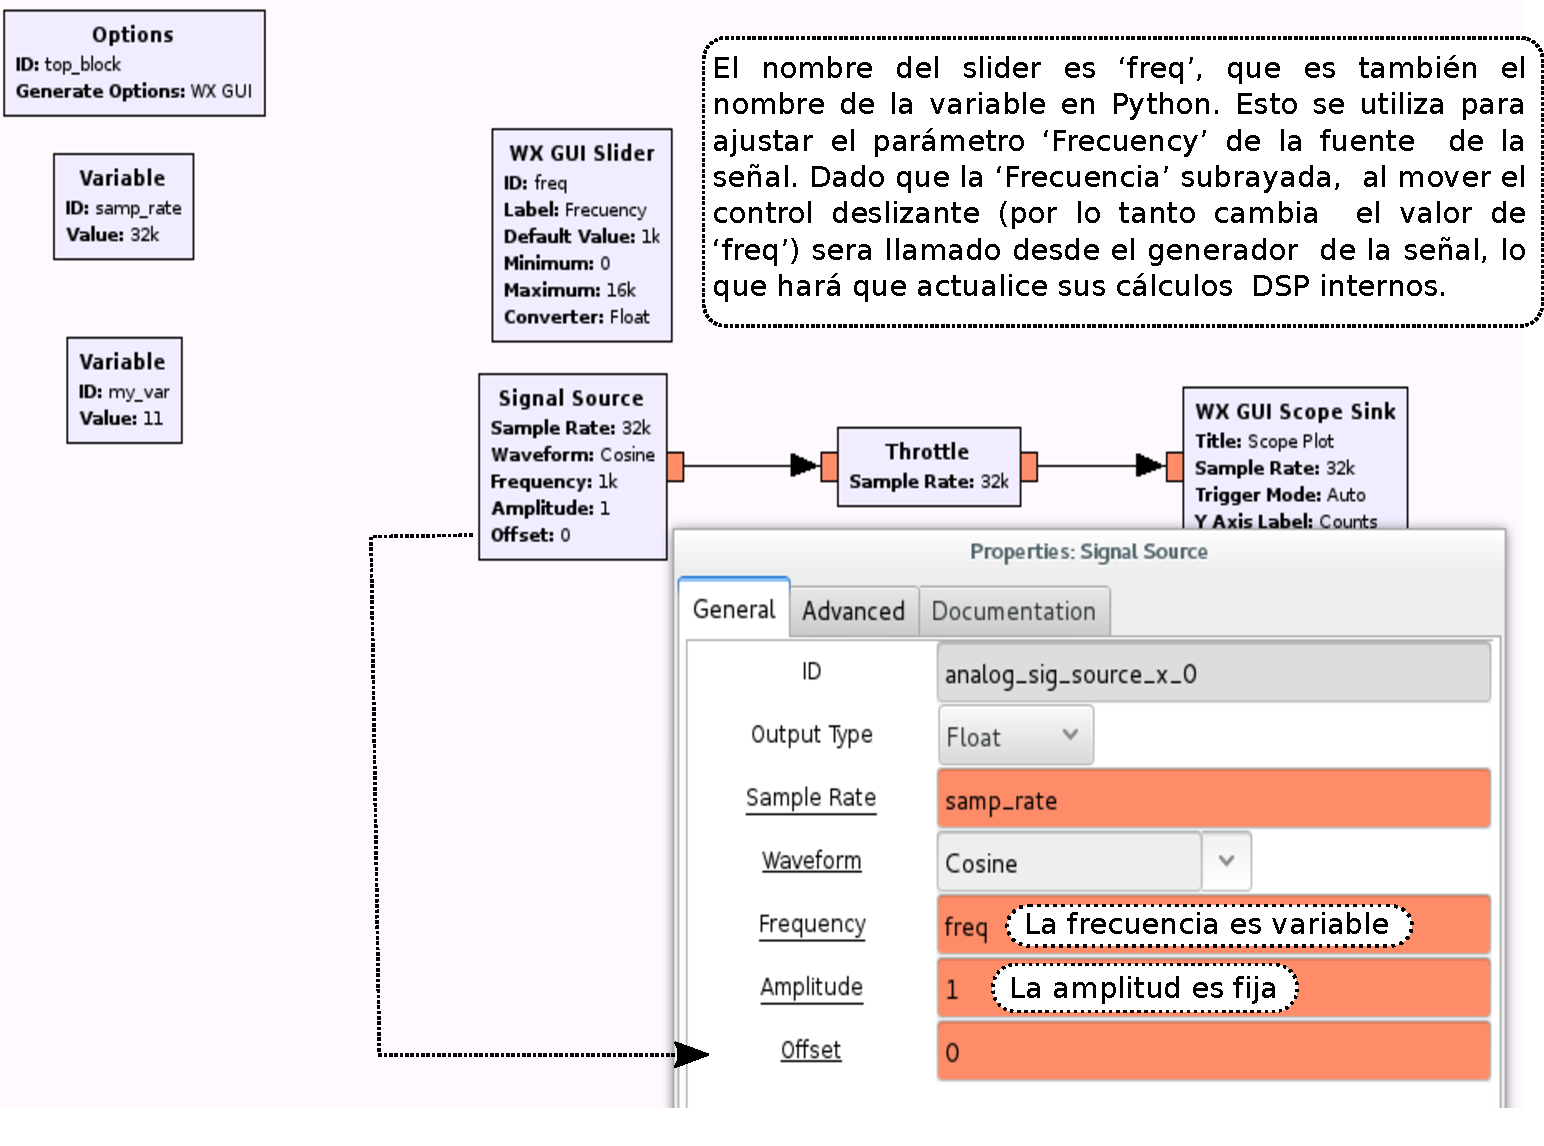
\includegraphics[width=.85\textwidth]{parte1/lab1/pdf/lab1_12.pdf}
\end{figure}
\end{frame}
%-----------------------------------

\begin{frame}{Primeros pasos }
\begin{figure}[H]
\vspace{-3mm}
\centering
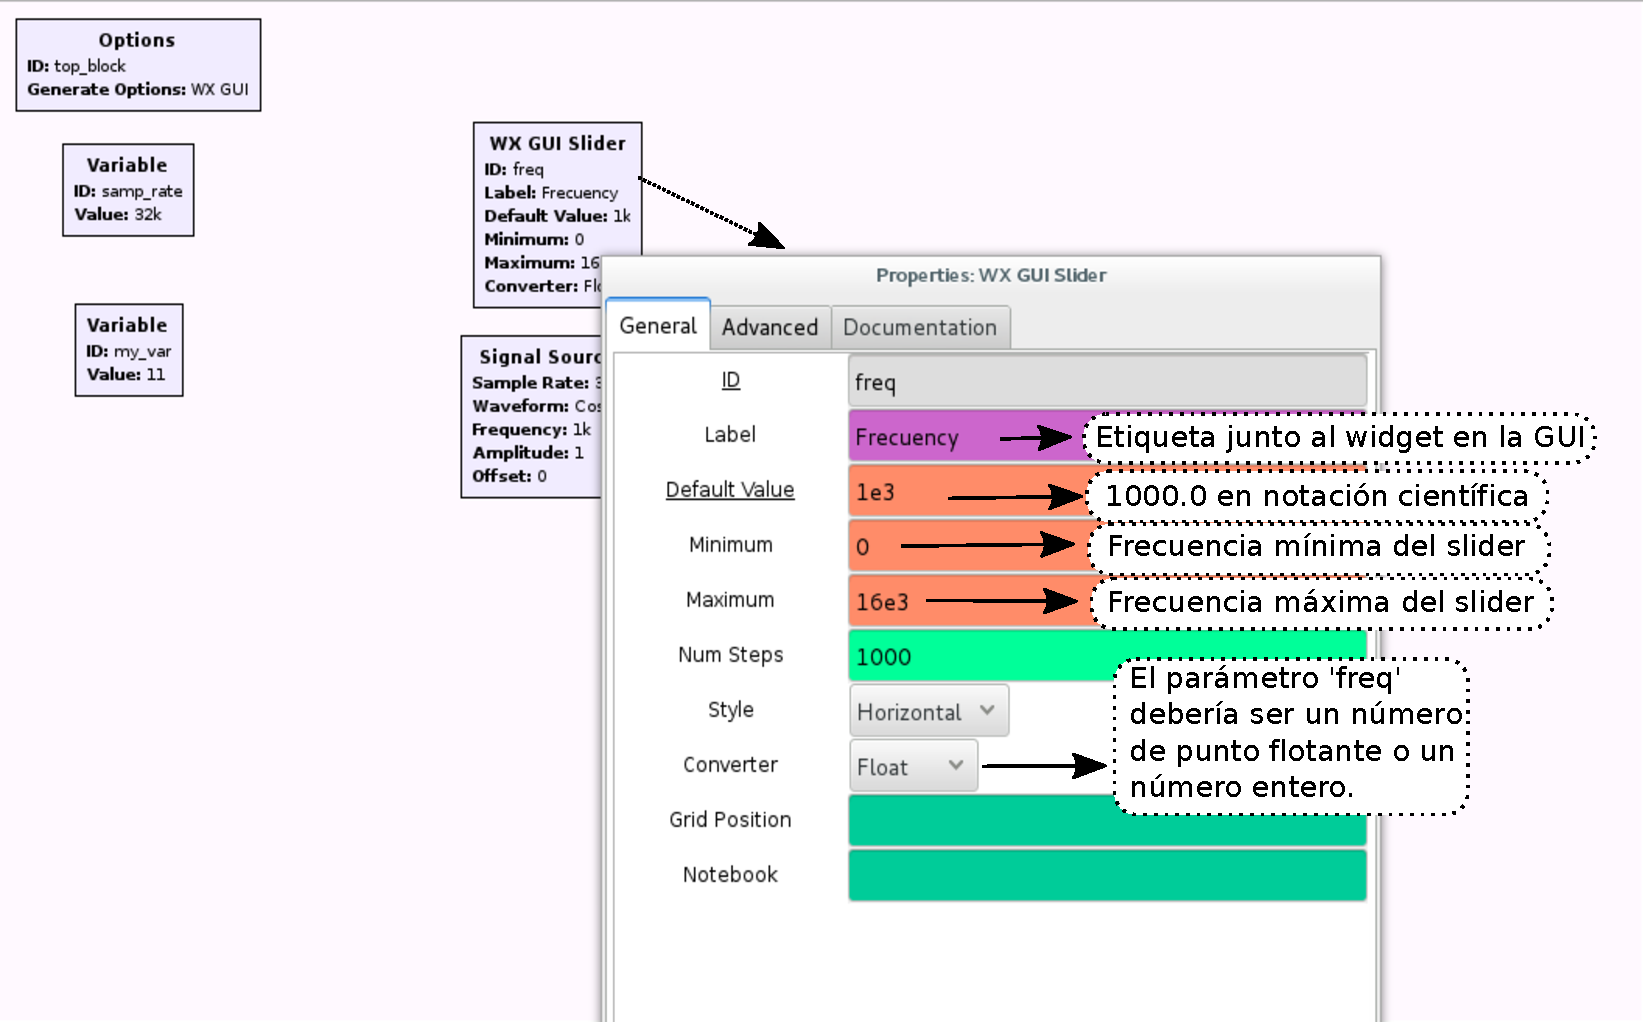
\includegraphics[width=\textwidth]{parte1/lab1/pdf/lab1_13.pdf}
\end{figure}
\end{frame}
%-----------------------------------

\begin{frame}{Primeros pasos }
\begin{figure}[H]
\vspace{-1cm}
\centering
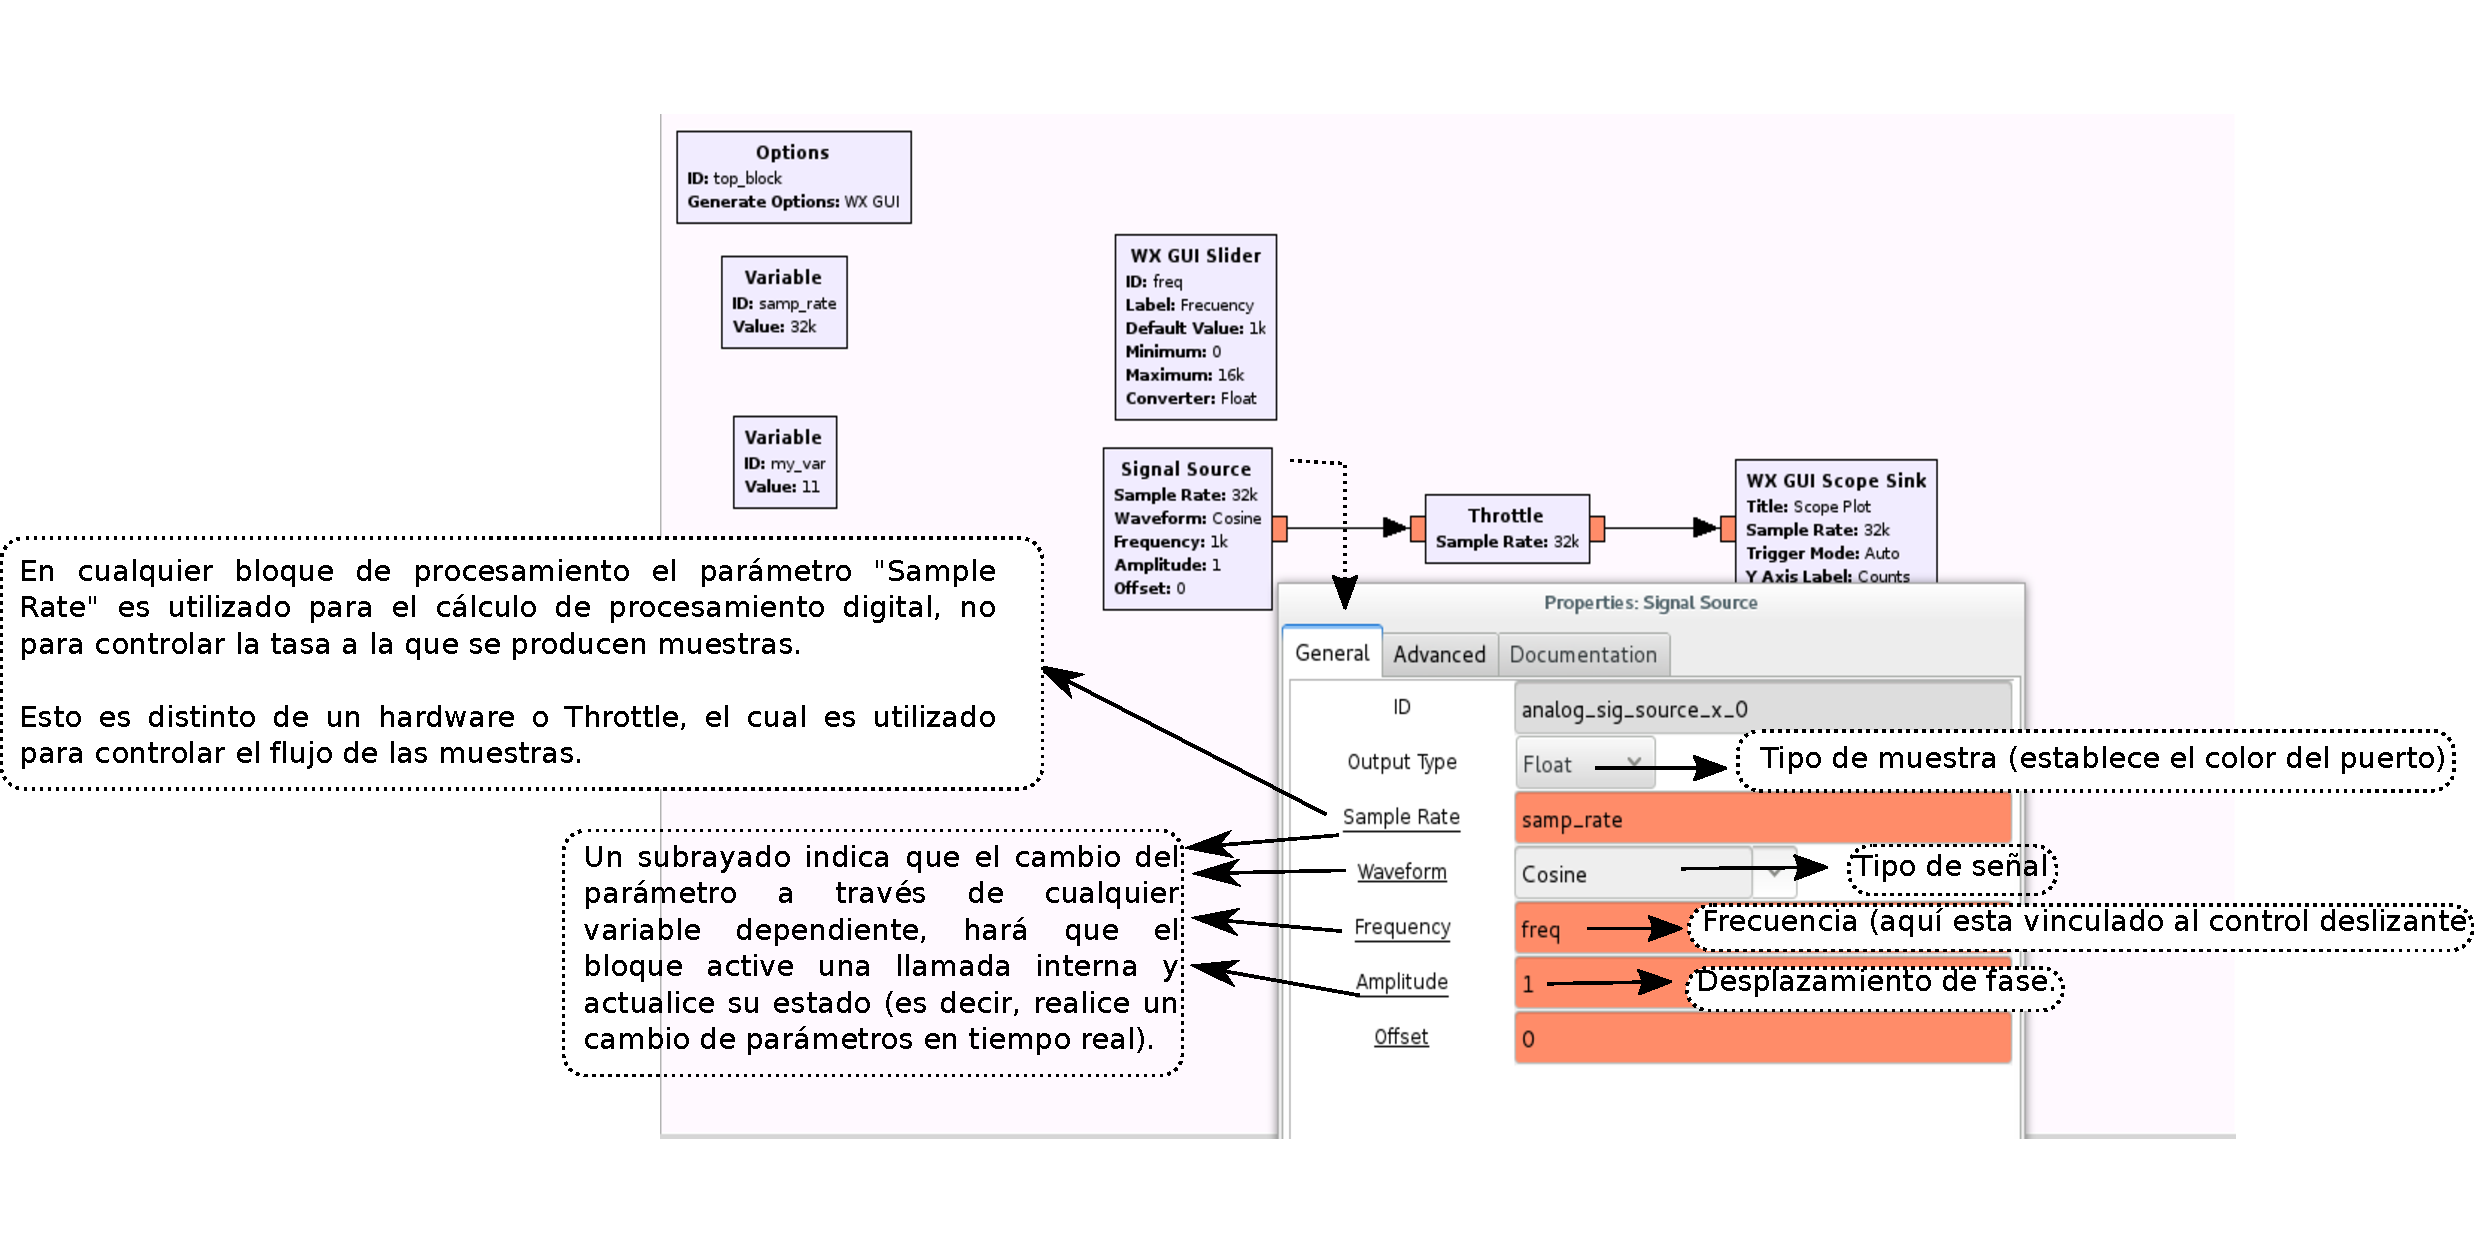
\includegraphics[width=1.05\textwidth]{parte1/lab1/pdf/lab1_14.pdf}
\end{figure}
\end{frame}
%-----------------------------------

\begin{frame}{Primeros pasos }
\begin{figure}[H]
\vspace{-3mm}
\centering
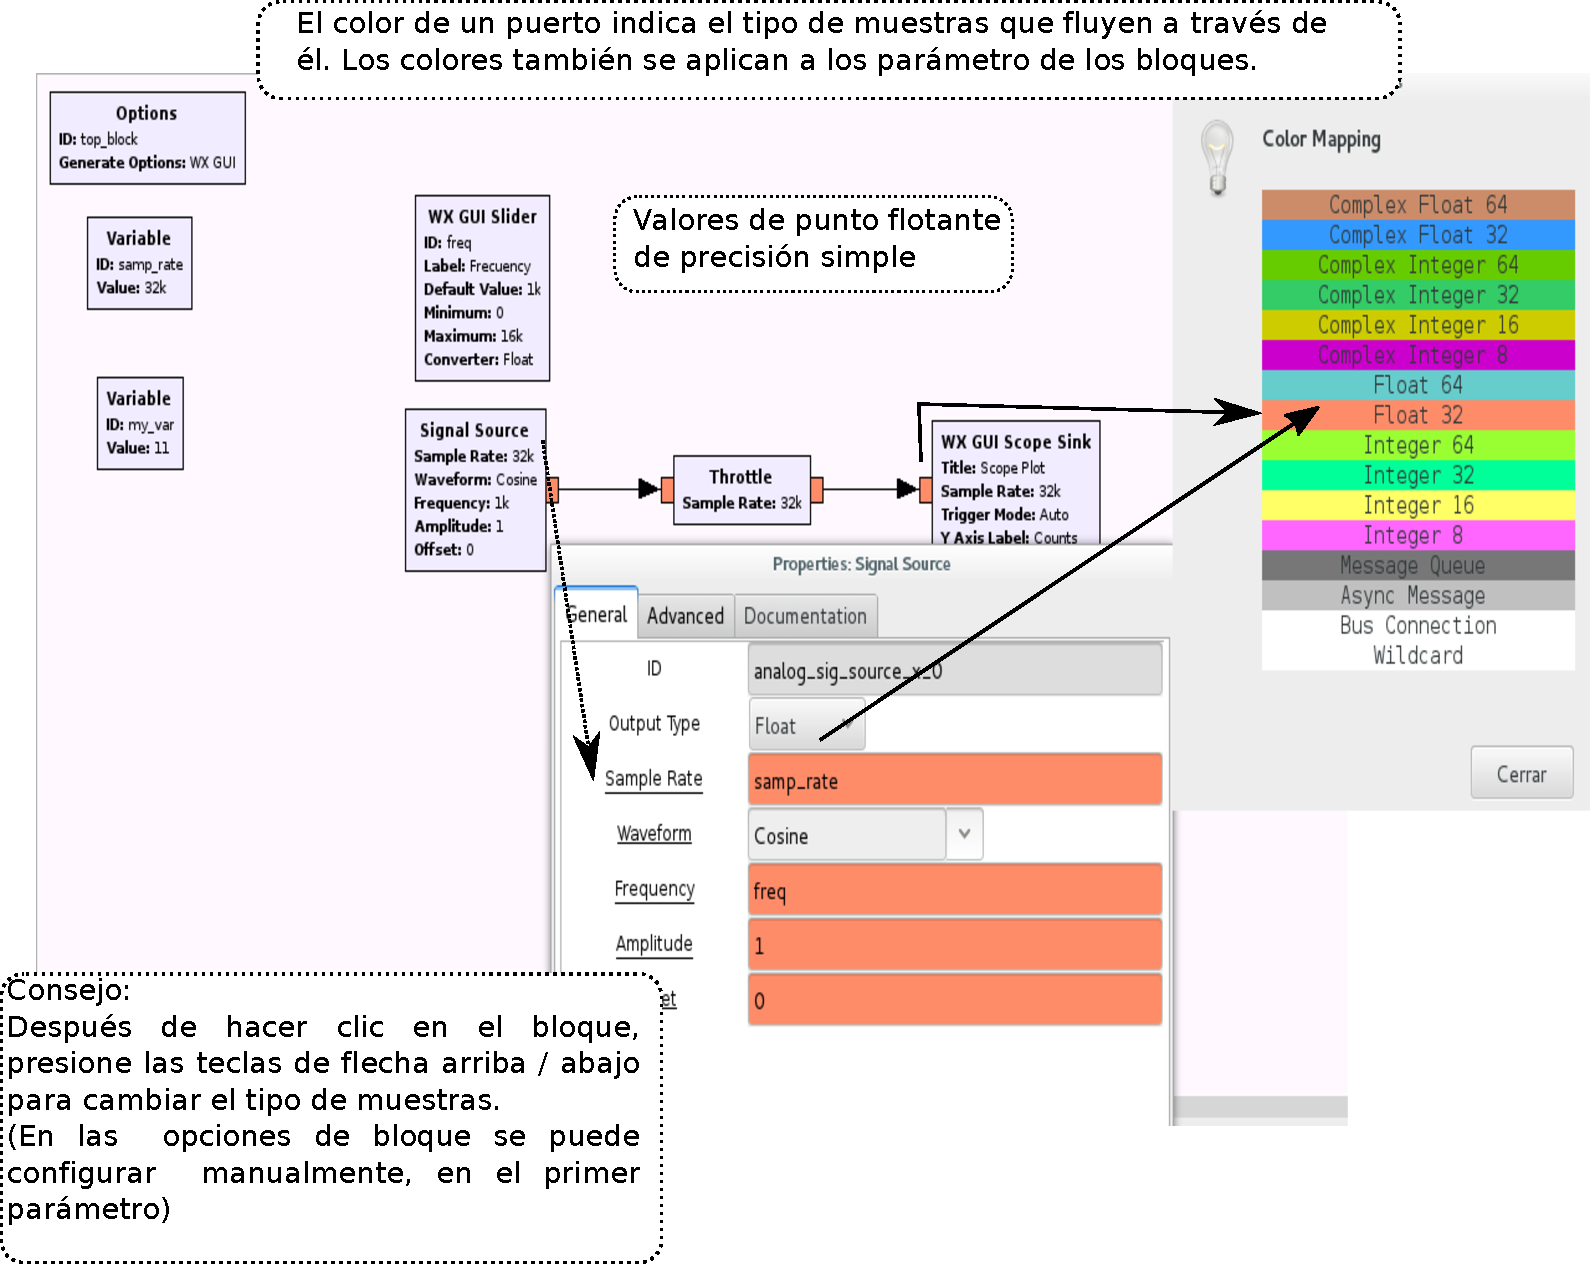
\includegraphics[width=.80\textwidth]{parte1/lab1/pdf/lab1_15.pdf}
\end{figure}
\end{frame}
%-----------------------------------

\begin{frame}{Primeros pasos }
\begin{figure}[H]
\centering
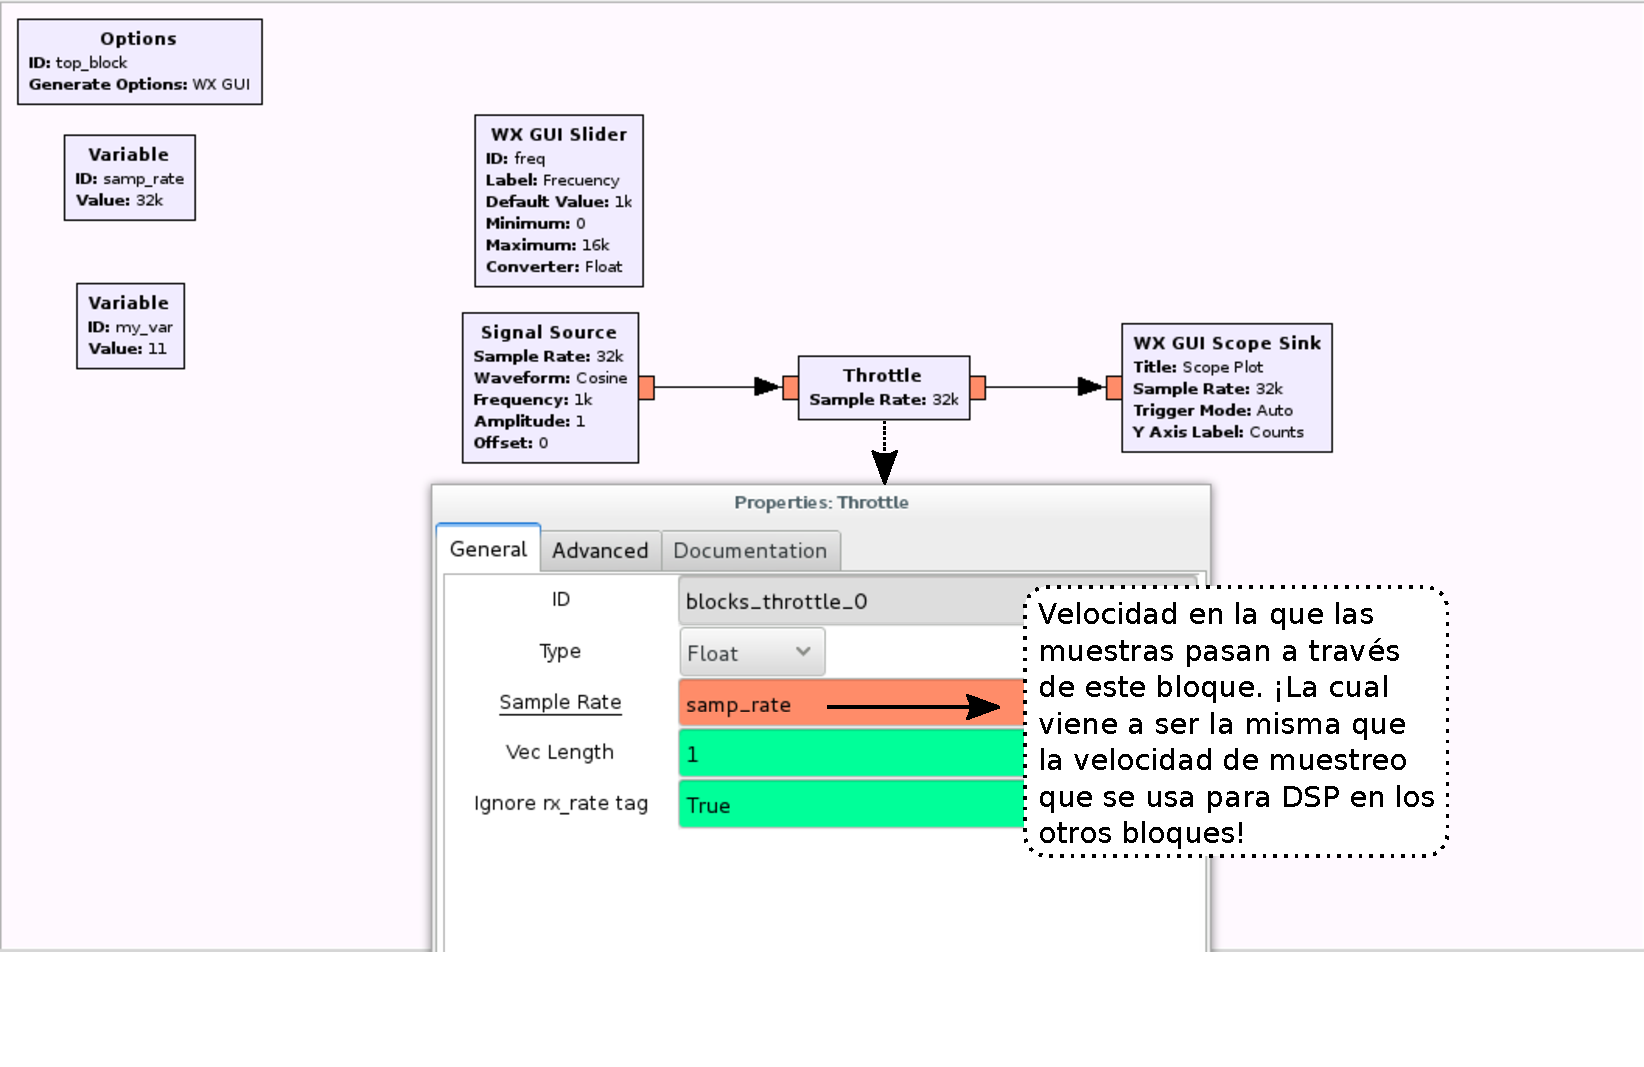
\includegraphics[width=\textwidth]{parte1/lab1/pdf/lab1_16.pdf}
\end{figure}
\end{frame}
%-----------------------------------

\begin{frame}{Primeros pasos }
\begin{figure}[H]
\vspace{-3mm}
\centering
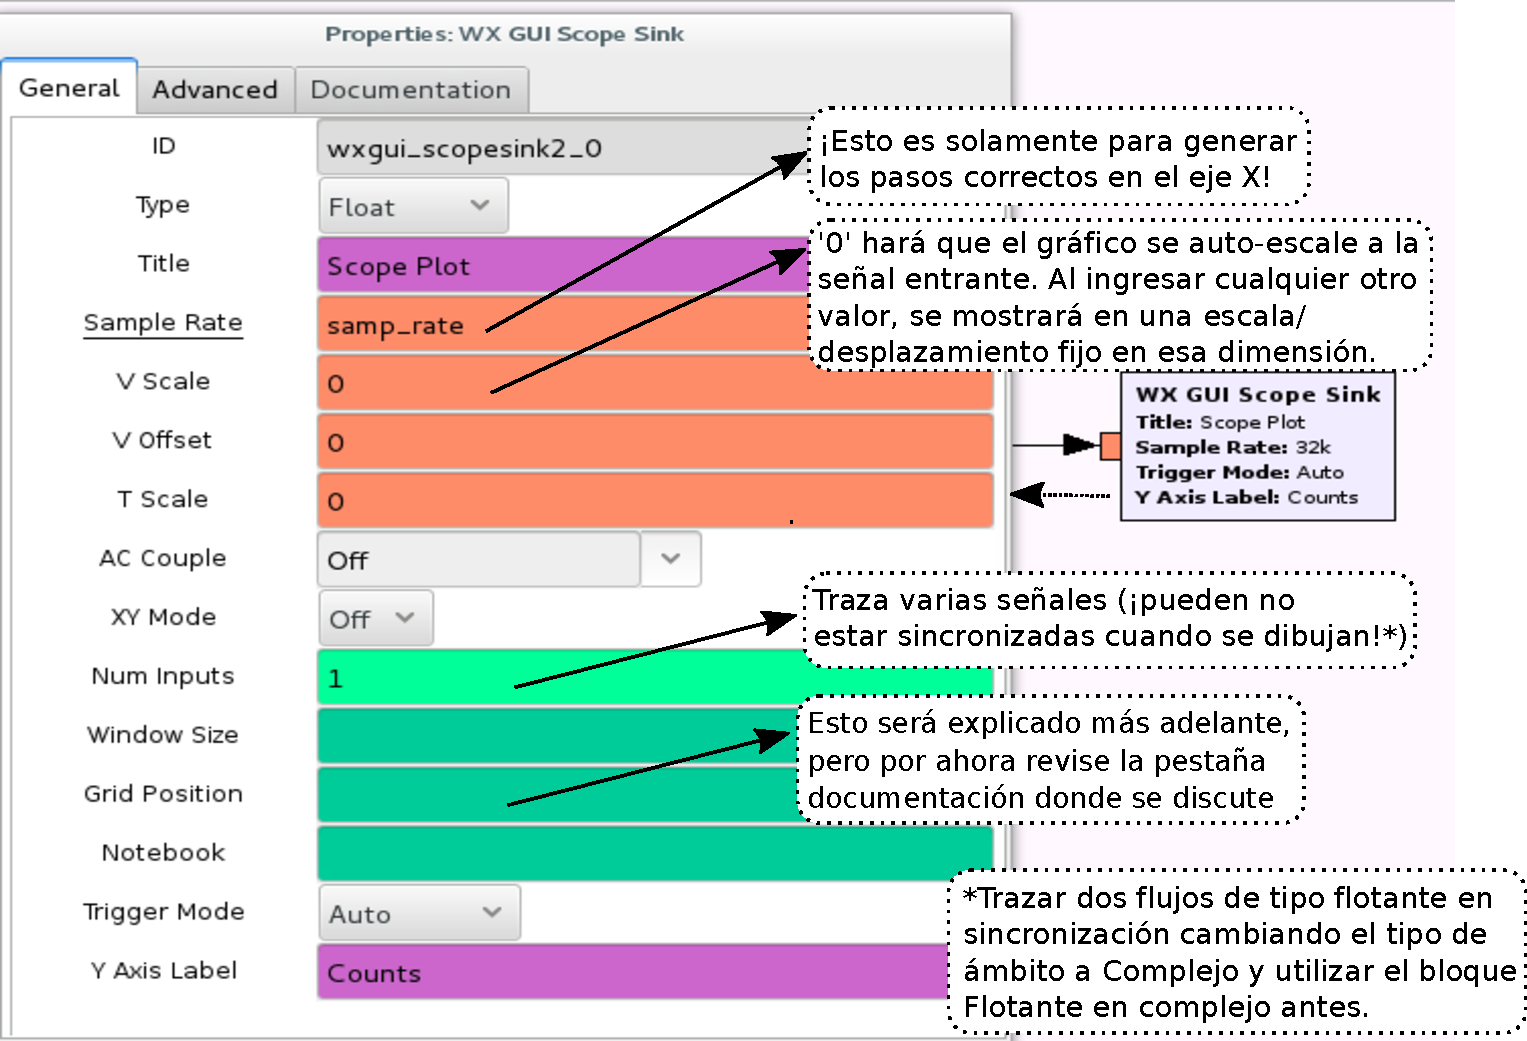
\includegraphics[width=.85\textwidth]{parte1/lab1/pdf/lab1_17.pdf}
\end{figure}
\end{frame}
%-----------------------------------

\begin{frame}{Primeros pasos }
\begin{figure}[H]
\centering
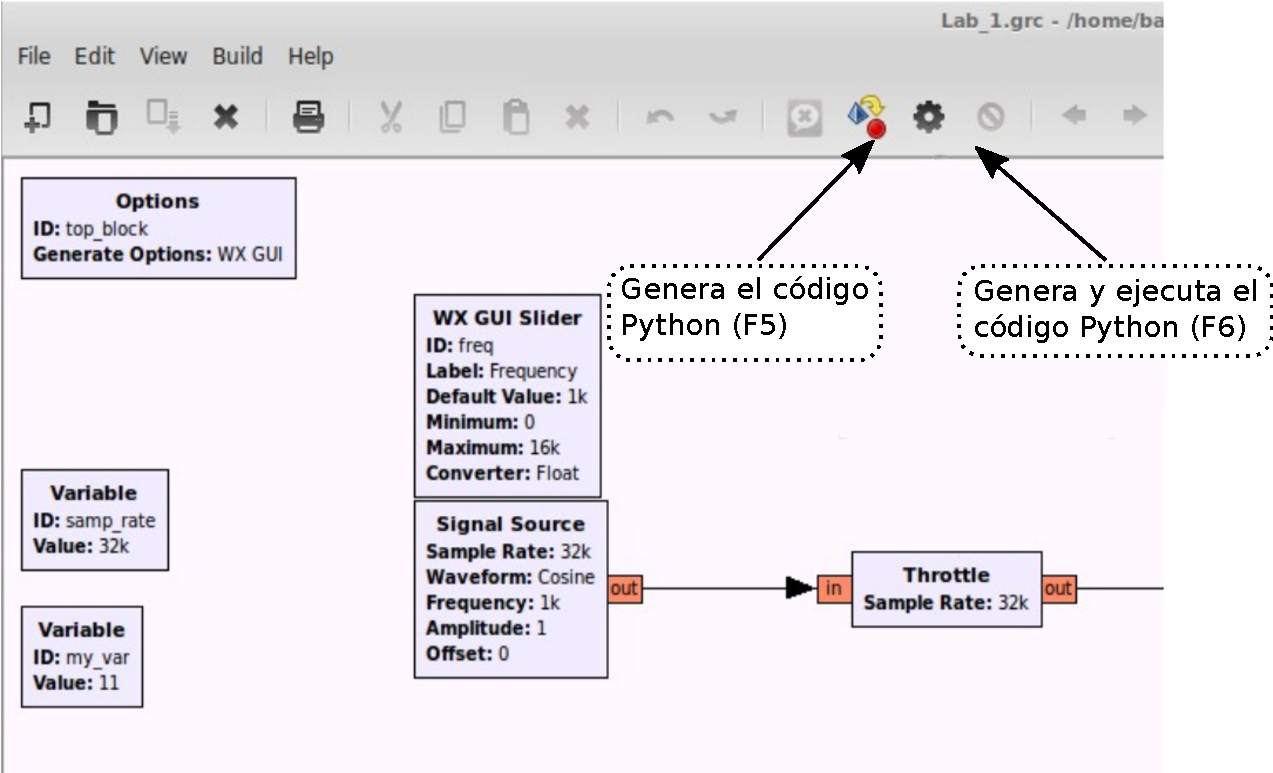
\includegraphics[width=\textwidth]{parte1/lab1/pdf/lab1_18.pdf}
\end{figure}
\end{frame}
%-----------------------------------

\begin{frame}{Primeros pasos }
Programa en Python generado por GRC
\begin{figure}[H]
\centering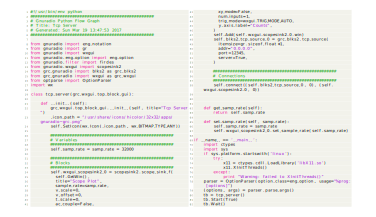
\includegraphics[width=0.95\textwidth]{parte1/lab1/pdf/lab1_18a.pdf}
\end{figure}
\end{frame}
%-----------------------------------

\begin{frame}{Primeros pasos }
\begin{figure}[H]
\centering
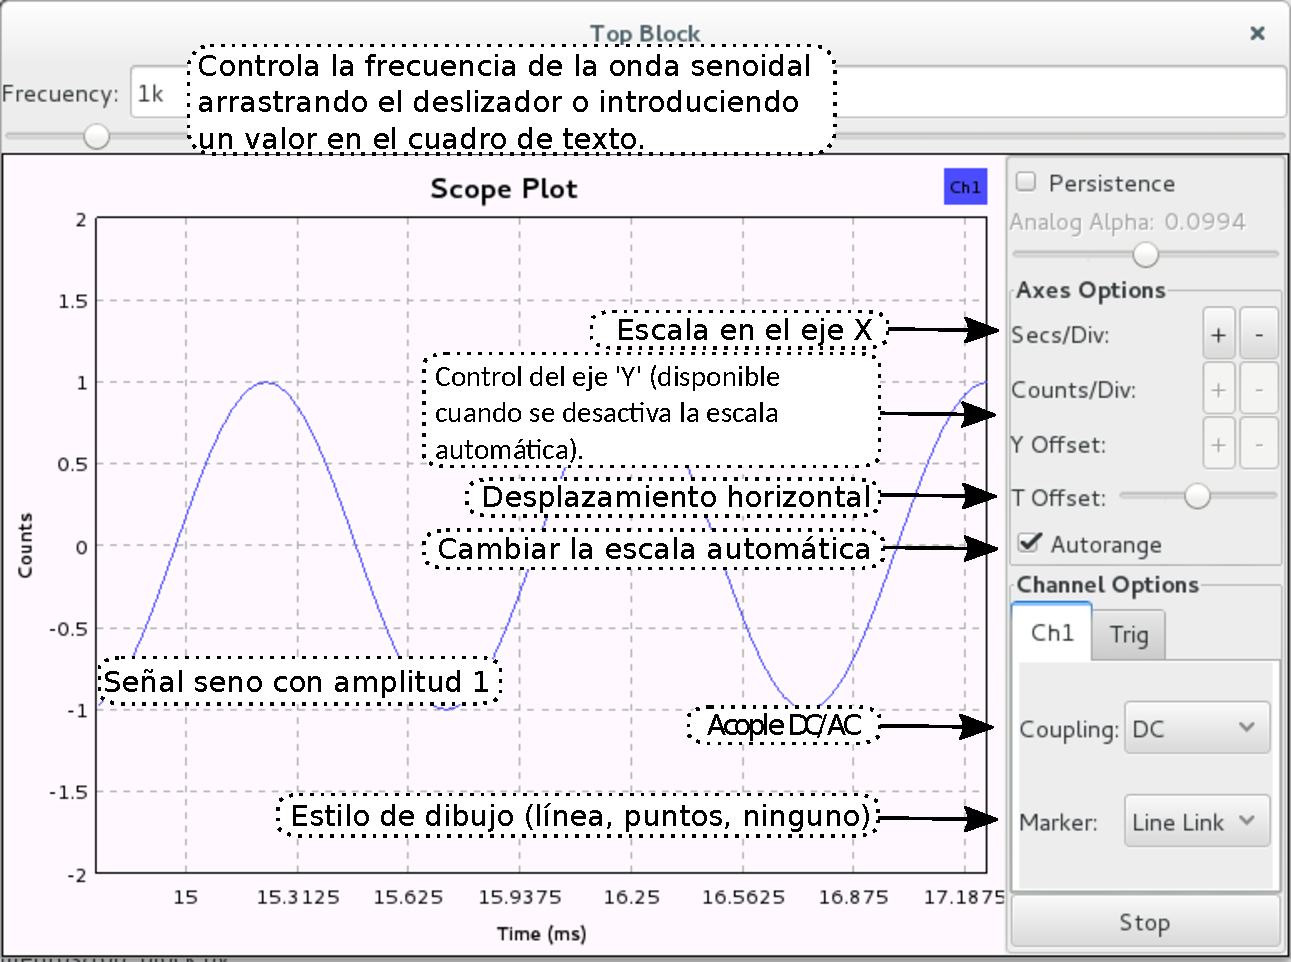
\includegraphics[width=\textwidth, height=0.55\textwidth]{parte1/lab1/pdf/lab1_19.pdf}
\end{figure}
\end{frame}
%-----------------------------------

\begin{frame}{Primeros pasos }
\begin{figure}[H]
\centering
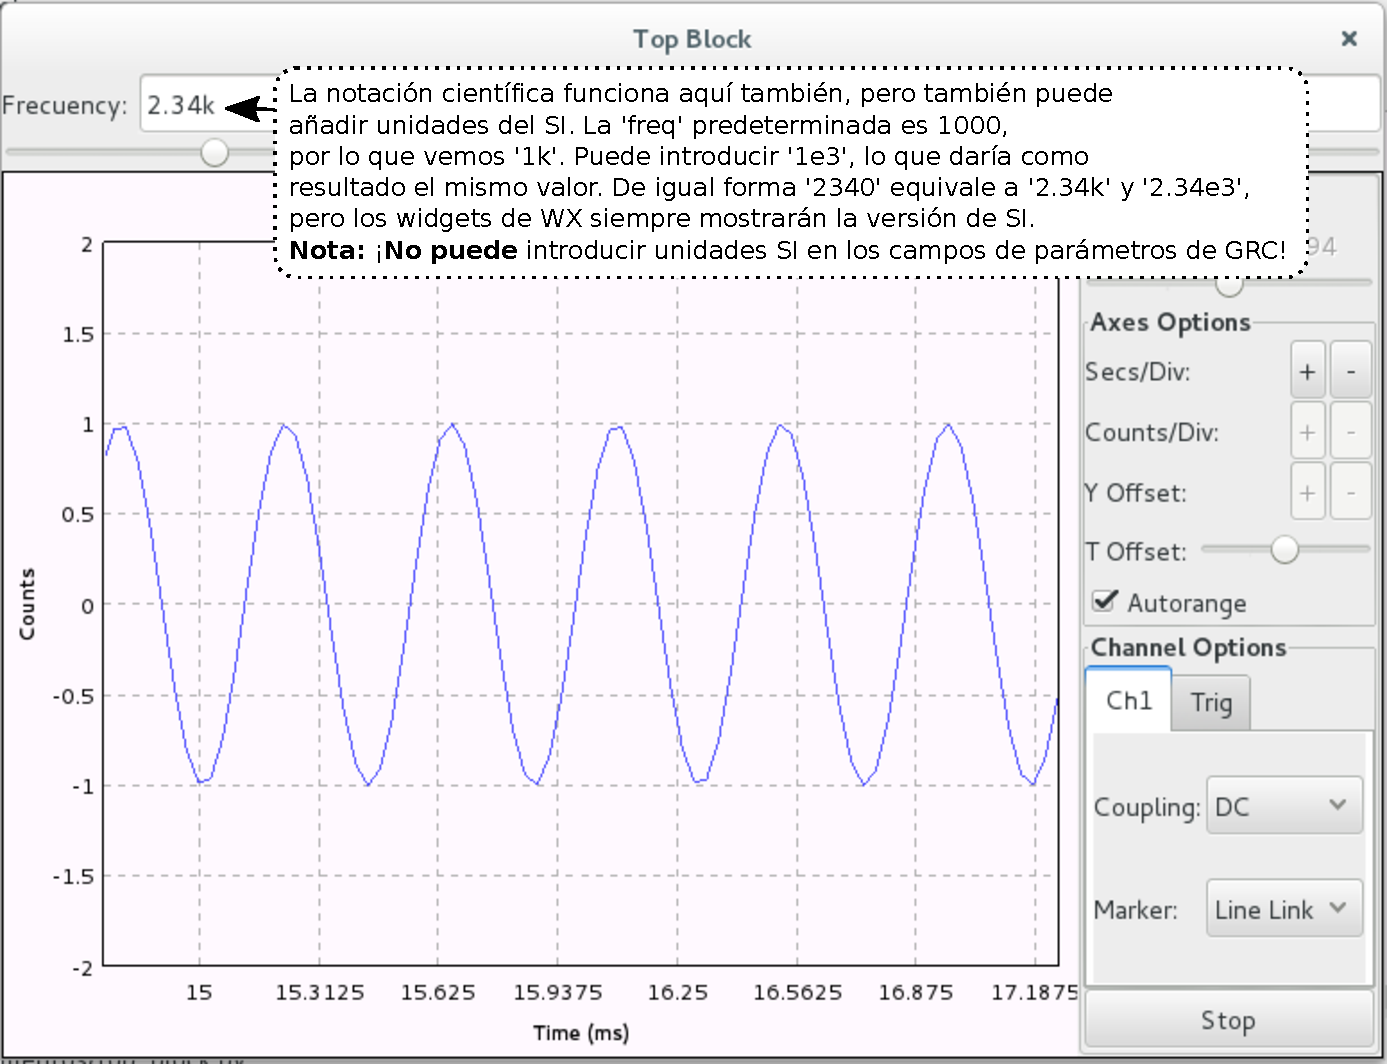
\includegraphics[width=\textwidth, height=0.55\textwidth]{parte1/lab1/pdf/lab1_20.pdf}
\end{figure}
\end{frame}
%-----------------------------------

\begin{frame}{Primeros pasos }
\begin{figure}[H]
\centering
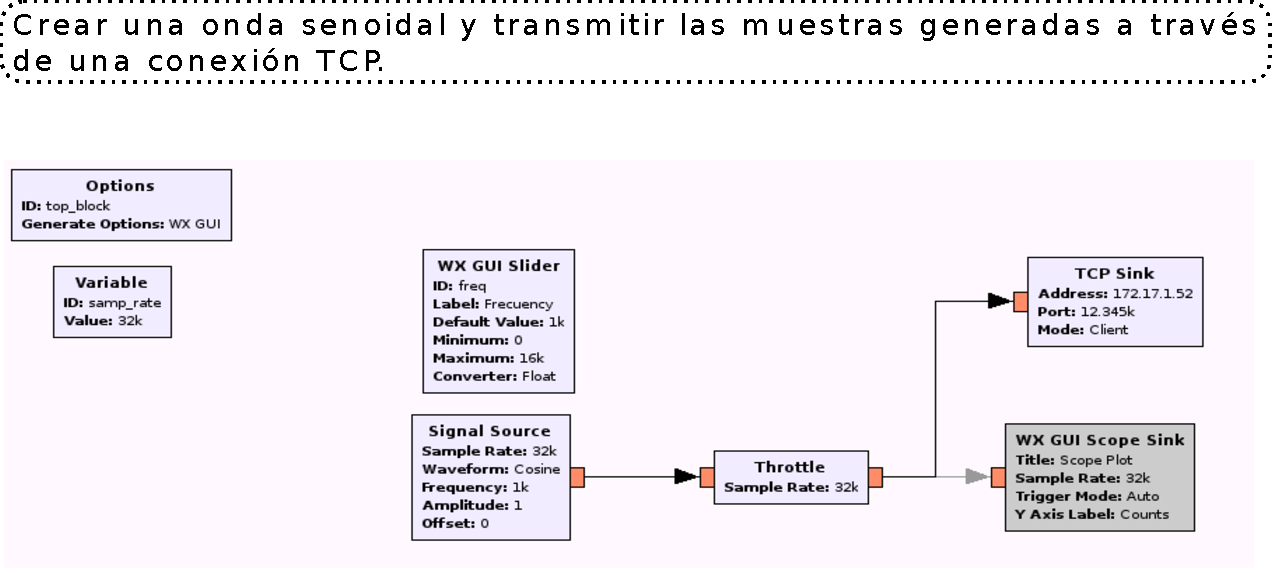
\includegraphics[width=\textwidth]{parte1/lab1/pdf/lab1_21.pdf}
\end{figure}
\end{frame}
%-----------------------------------

\begin{frame}{Primeros pasos }
\begin{figure}[H]
\centering
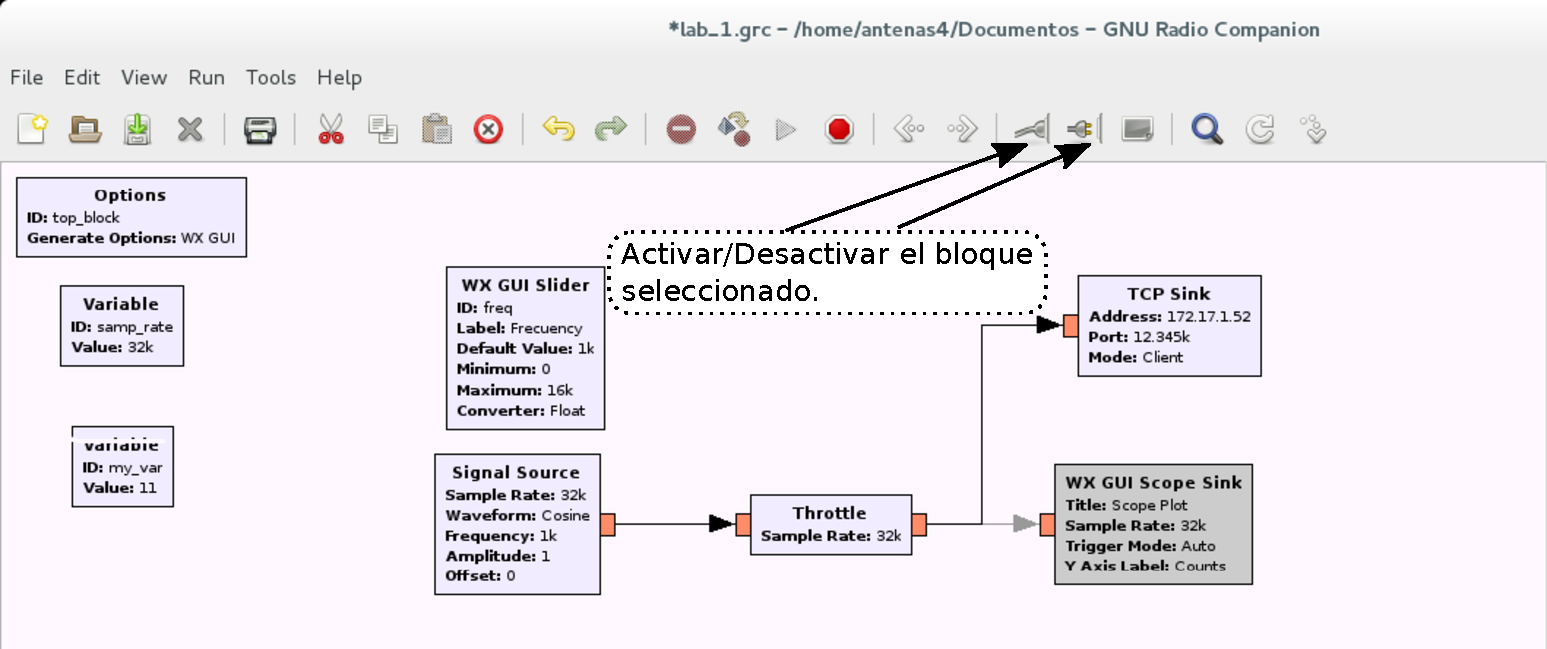
\includegraphics[width=\textwidth]{parte1/lab1/pdf/lab1_22.pdf}
\end{figure}
\end{frame}
%-----------------------------------

\begin{frame}{Primeros pasos }
\begin{figure}[H]
\centering
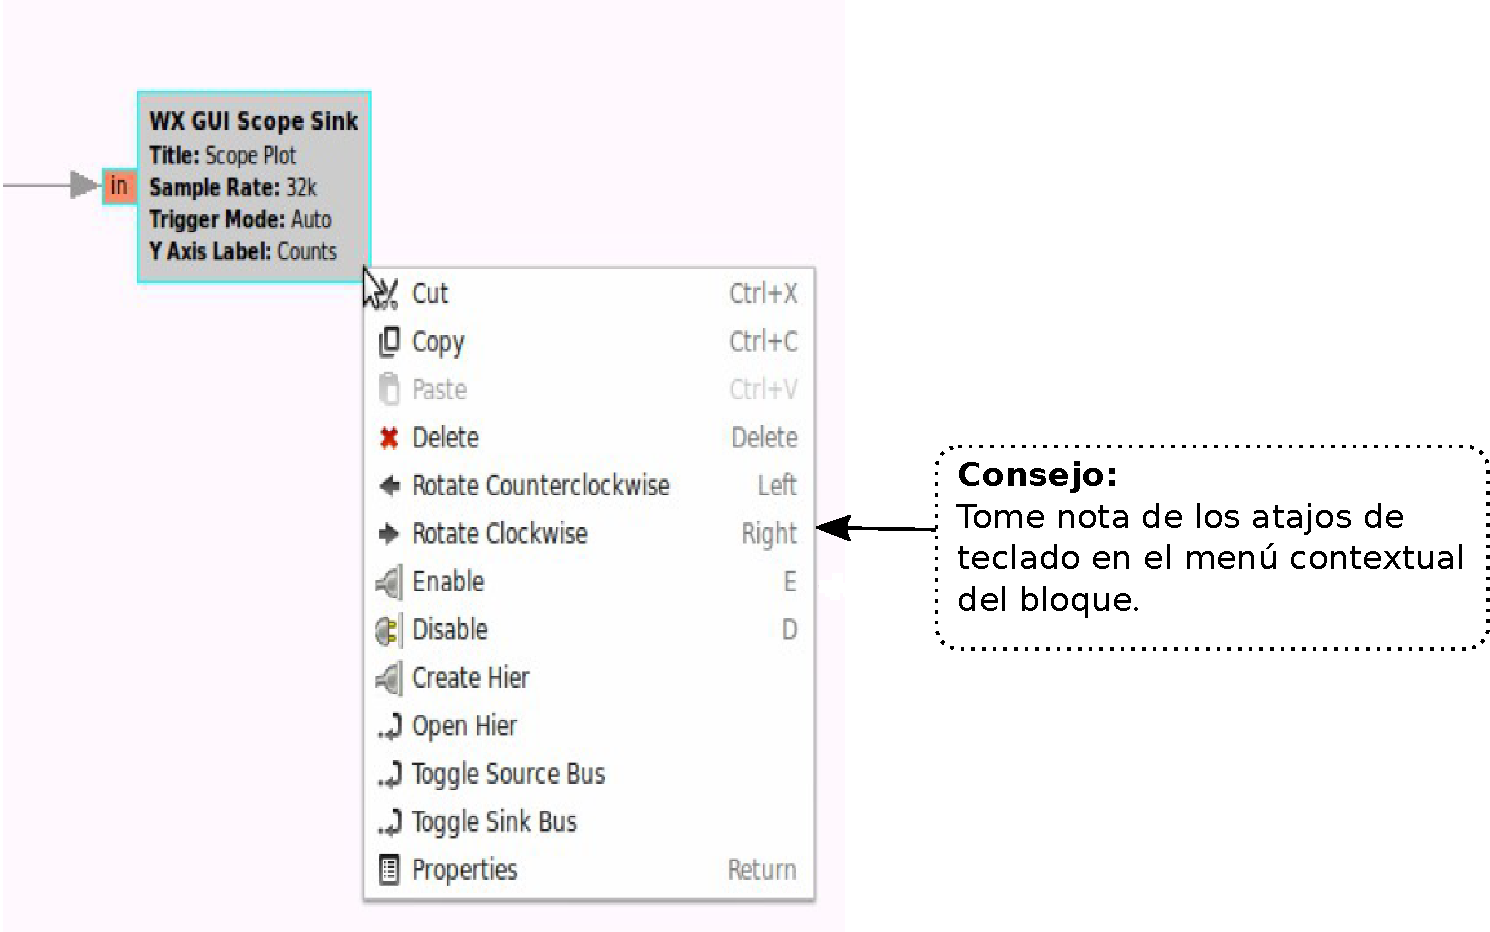
\includegraphics[width=\textwidth, height=0.6\textwidth]{parte1/lab1/pdf/lab1_23.pdf}
\end{figure}
\end{frame}
%-----------------------------------

\begin{frame}{Primeros pasos }
\begin{figure}[H]
\centering
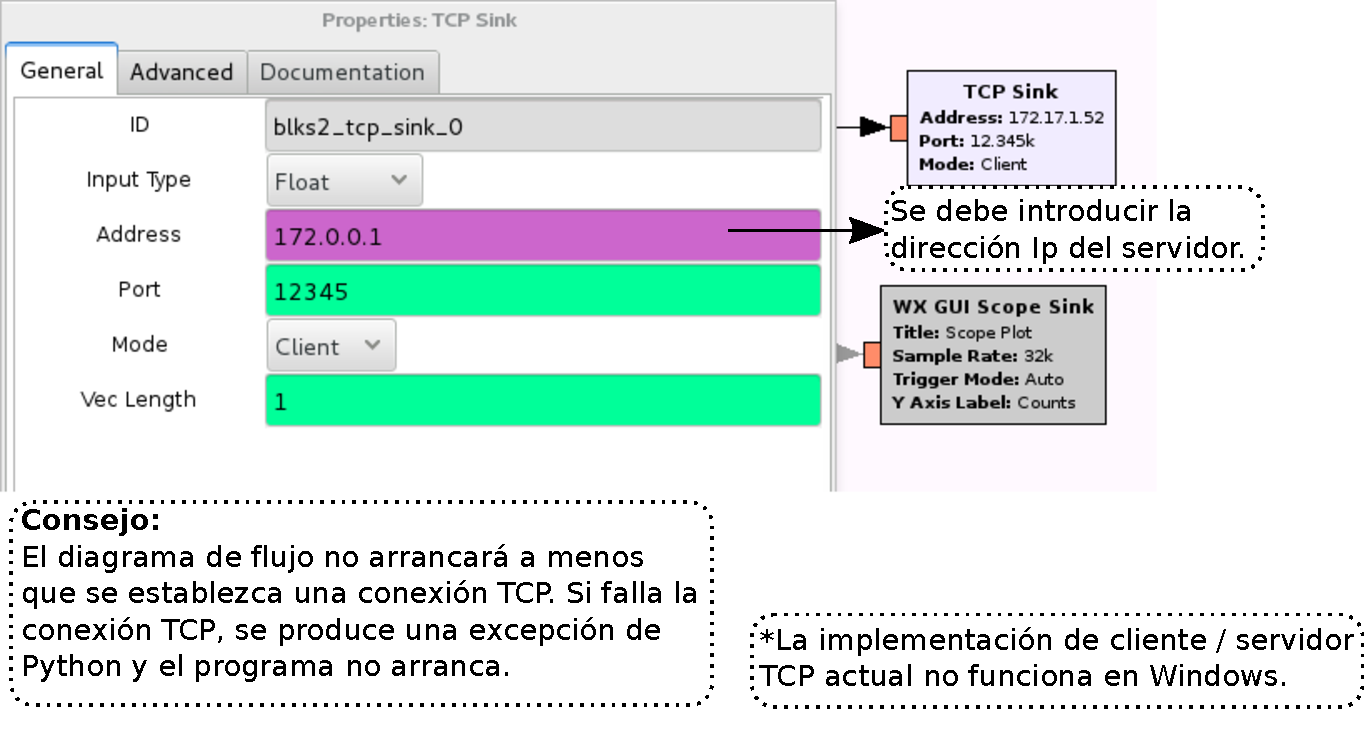
\includegraphics[width=\textwidth]{parte1/lab1/pdf/lab1_24.pdf}
\end{figure}
\end{frame}
%-----------------------------------

\begin{frame}{Primeros pasos }
\begin{figure}[H]
\centering
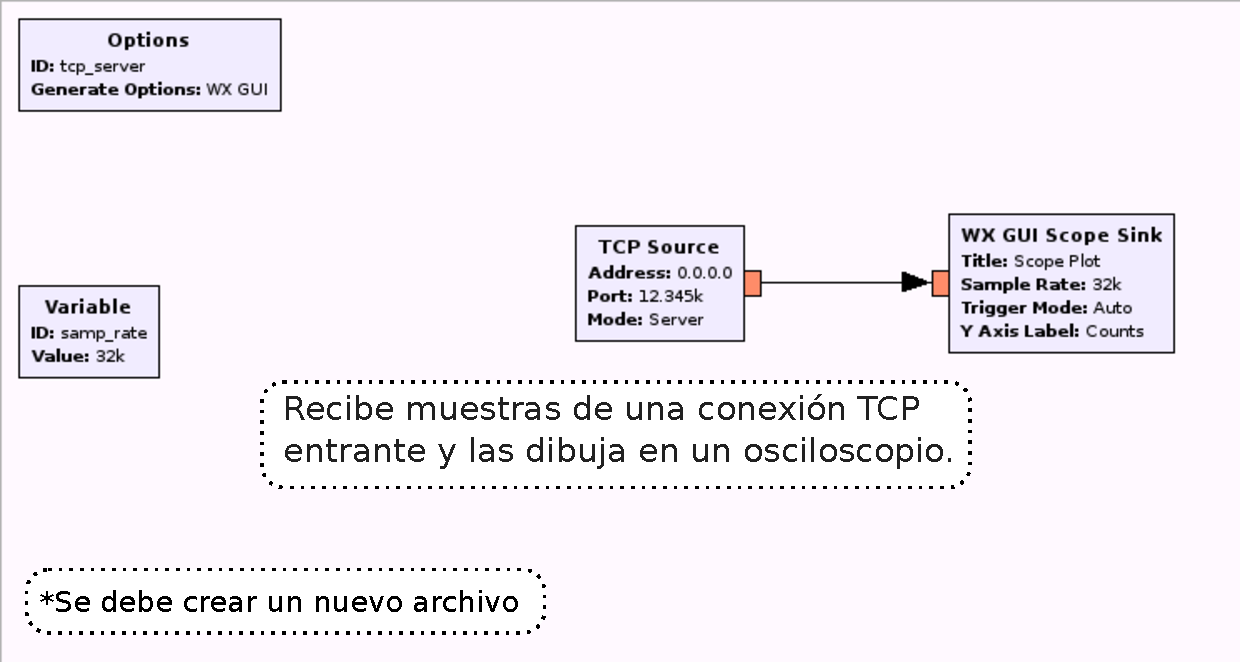
\includegraphics[width=\textwidth]{parte1/lab1/pdf/lab1_25.pdf}
\end{figure}
\end{frame}
%-----------------------------------

\begin{frame}{Primeros pasos }
\begin{figure}[H]
\centering
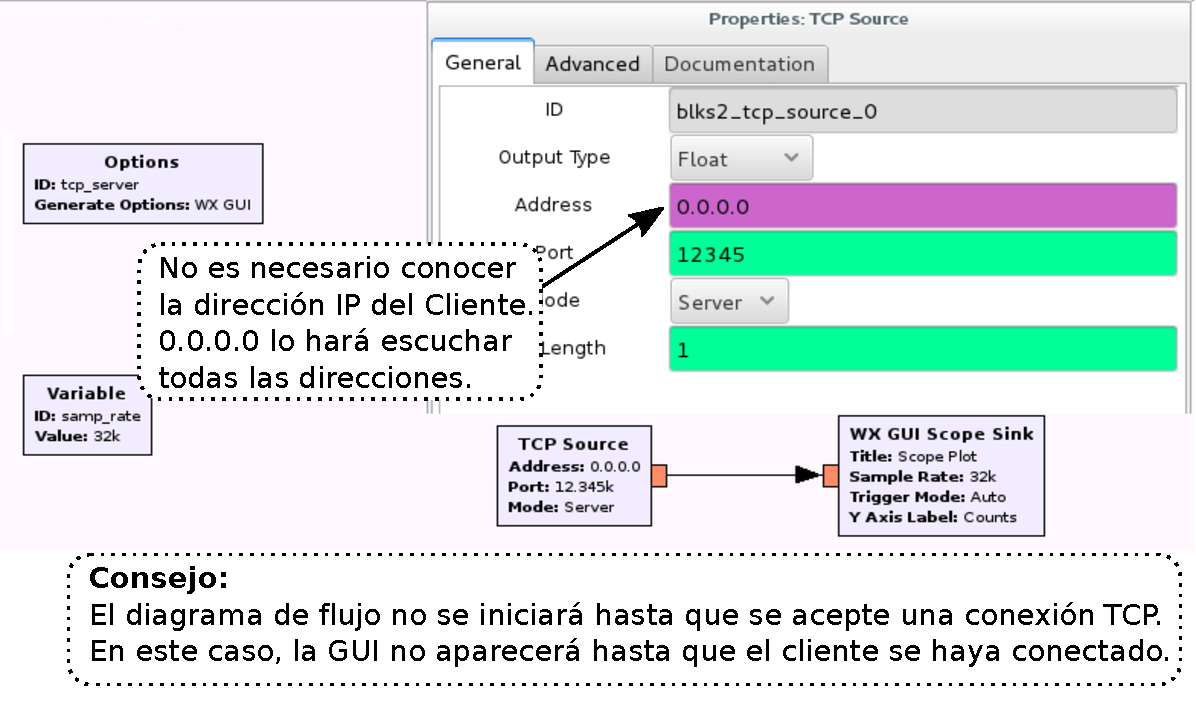
\includegraphics[width=\textwidth]{parte1/lab1/pdf/lab1_26.pdf}
\end{figure}
\end{frame}
%-----------------------------------

\begin{frame}{Primeros pasos }
\begin{figure}[H]
\centering
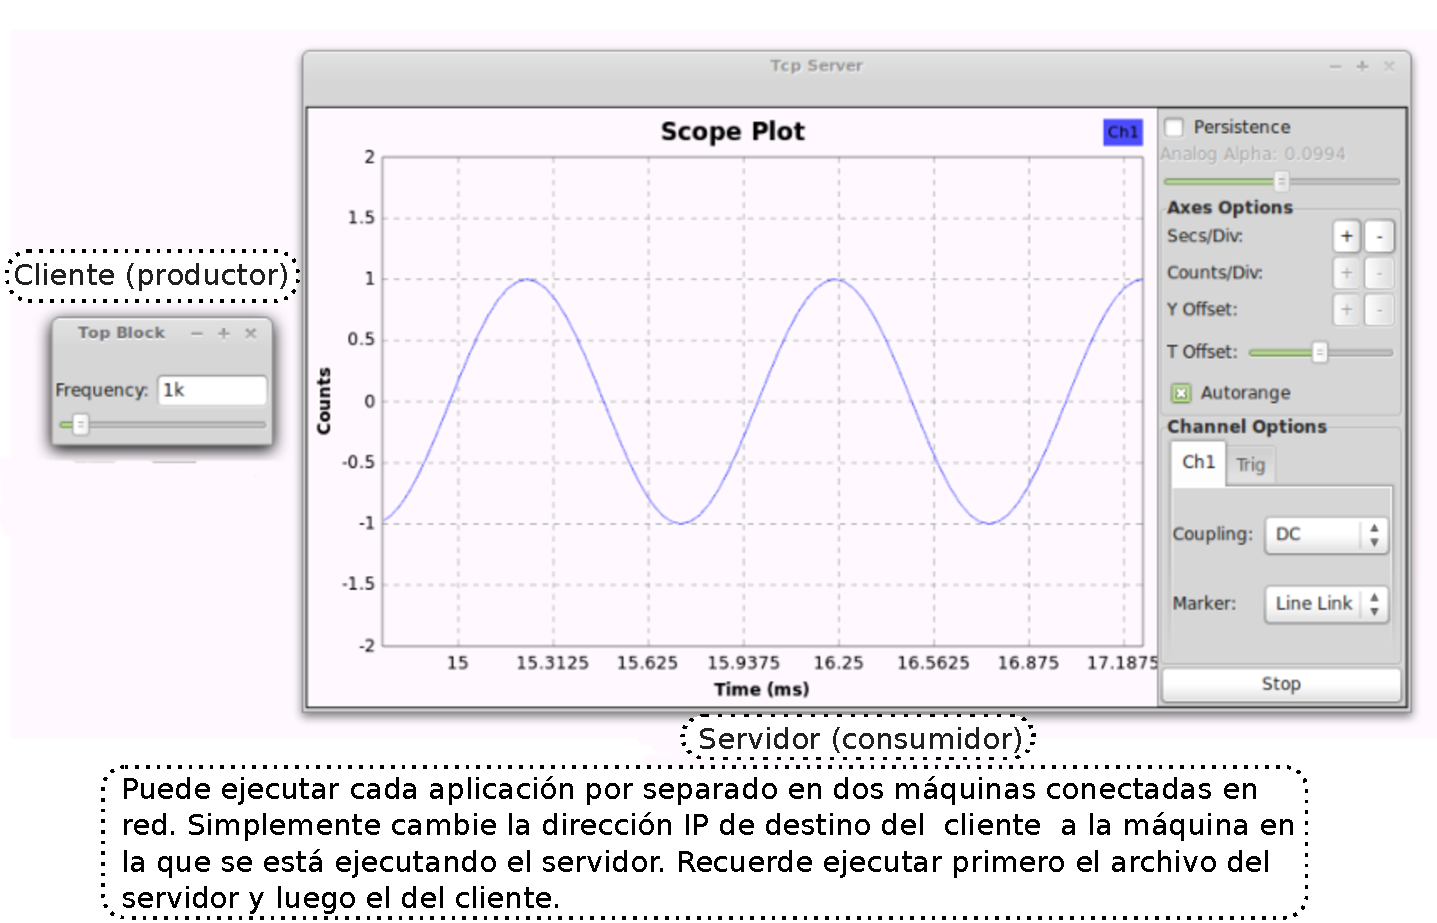
\includegraphics[width=\textwidth, height=0.55\textwidth]{parte1/lab1/pdf/lab1_27.pdf}
\end{figure}
\end{frame}
%-----------------------------------

\subsubsection{Actividad 1_lab1}
\begin{frame}

\pgfdeclareimage[width=\paperwidth,height=\paperheight]{bg}{imagenes/fondo_seccion}
\setbeamertemplate{background}{\pgfuseimage{bg}}

\definecolor{greenU}{RGB}{212,202,72}
\setbeamercolor{block body}{fg=Black,bg=greenU}
\begin{block}{}
	\centering
	%\vspace{1mm}
	\Large{\textit{Actividades}}
	%\vspace{1mm}
\end{block}
\end{frame}

\begin{frame}

\pgfdeclareimage[width=\paperwidth,height=\paperheight]{bg}{imagenes/fondo3}
\setbeamertemplate{background}{\pgfuseimage{bg}}

\frametitle{\underline{\textbf{Transmisión de señales por multiplexación}}}

En esta actividad usted debe transmitir 3 señales periódicas por medio del TCP (Protocolo de 	Control de Transmisión) desde el cliente, mediante el proceso de multiplexación de señales, al 	servidor, que se encargará de demultiplexar la señal recibida y mostrar las 3 que fueron  	transmitidas en el Scope Sink.\vspace{2mm}

Es importante saber que:
\begin{enumerate}[1.]
\item {La multiplexación es el proceso mediante el cual diferentes mensajes de información (Señales) se combinan en una única señal con el fin de trasmitirla. }\\

\item {La demultiplexación es el proceso mediante el cual la señal multiplexada recibida se divide en cada una de las señales que la generaron.}\\
\end{enumerate}
\end{frame}

%-----------------------------------

\begin{frame}

\pgfdeclareimage[width=\paperwidth,height=\paperheight]{bg}{imagenes/fondo3}
\setbeamertemplate{background}{\pgfuseimage{bg}}

\frametitle{\underline{\textbf{Pistas para la actividad}}}

Las pistas son:
\begin{enumerate}[1.]
	\item {Modo cliente: Bloques y conexiones de los primeros pasos. (WX GUI Slider, Signal Source, TCP Sink, Scope Sink, Throttle, Stream Mux, Variable)}
	
	\item {Modo servidor:  Bloques y conexiones de los primeros pasos. (TCP Source, Scope Sink, Stream to Streams)}
	\item {Multiplexación: Bloque Stream Mux. En el parámetro Lengths se debe agregar el número de ítems de cada señal, en forma de lista. Para la actividad las señales cuentan con un solo ítem. 
	Como ejemplo de lo anterior tenemos que: }
\begin{itemize}
	\item 2 señales = 1,1    
	\item 3 señales = 1,1,1 
	\item 4 señales = 1,1,1,1
\end{itemize}
	\item {Demultiplexación: Bloque Stream to Streams.}
    \item { El tipo de dato en todos los bloques debe ser el mismo. (float)}
	\item {Habilitar las entradas o salidas suficientes para los bloques.}
\end{enumerate}
\end{frame}

%-----------------------------------

%\begin{frame}{Actividad de los Primeros pasos }
%\begin{figure}[H]
%\centering
%\vspace{-3mm}
%\includegraphics[width=0.9\textwidth]{parte1/lab1/Actividades/pdf/prueba.pdf}
%\end{figure}
%\end{frame}
%-----------------------------------

\subsubsection{Actividad2}


\begin{frame}
	\frametitle{\underline{\textbf{Modificación de las variables de una señal periódica}}}
	
	Aprender a variar los componentes básicos de una señal periódica (amplitud, frecuencia, fase y nivel DC) en GNU Radio.\vspace{2mm}
	
	Es importante saber que:
	
	\begin{enumerate}[1.]
		\item{La forma más simple de representar una señal periódica es una senoidal como se presenta matemáticamente a continuación}\\
		
		$$x(t)=A\sin(2 \pi f + \phi) + K$$\\
		
		En donde:\\
		
		\item{Amplitud ($A$): Es el valor máximo que toma la señal, es decir, la distancia entre el punto máximo de la señal y cero, este punto puede ser tanto positivo como negativo.}\\
		
		\item{Frecuencia ($f$): Es el número de ciclos que realiza la señal por unidad de tiempo, esta medida está dada en Hertz (Hz), que equivale a un ciclo por segundo, lo que significa que 80 Hz son 80 ciclos por cada segundo que transcurre.}\\
		
	\end{enumerate}
\end{frame}


\begin{frame}
	\frametitle{\underline{\textbf{Modificación de las variables de una señal periódica}}}
	\begin{enumerate}[1.]
		
		\item{La fase ($\phi$): Indica la magnitud de una de variación ciclíca, siendo la fracción del período que transcurre desde el instante tomado al estado hasta la referencia, es decir el desplazamiento que tiene una señal en grados con respecto a su referencia.}\\
		
		\item{Nivel DC ($K$): Es el valor medio de la señal, lo que quiere decir que es un voltaje en DC que se le suma a la señal AC, para obtener un desplazamiento en la amplitud de la señal, puede ser tanto positivo como negativo.}\\
		
	\end{enumerate}
\end{frame}

\begin{frame}{Actividad}
	\begin{enumerate}[1.]
		
		\item{Realizar un programa que permita variar los componentes básicos de una señal periódica (amplitud, frecuencia, fase y nivel DC) en GNU Radio.}\\
		
	\end{enumerate}
\end{frame}

\begin{frame}
	
	\frametitle{\underline{\textbf{Pistas para la actividad}}}
	
	Las pistas son:
	\begin{enumerate}[1.]
		
		\item {Repasar los bloques utilizados en la primera guía "Primeros pasos"}\\
		\item {Debe existir un WX GUI Slider para cada variable que se desee modificar en el osciloscopio.}\\
		\item {Para una mejor apreciación  de los cambios en las variables de la señal se sugiere añadir otra señal que sirva como referencia}\\
		\item {Coherencia entre los tipos de dato entre bloques}\\
		\item {Para variar el nivel DC de la señal, el oscilocopio debe tener la opción "Coupling" en DC}\\
		\item {Para poder configurar correctamente la fase se debe dejar una frecuencia fija, se agrega un bloque "Delay" y en este bloque se representa la formula de la fase de la siguirnte forma: \\
(Fase * Samp\_rate)/360/Frecuencia }
	\end{enumerate}
\end{frame}

